\documentclass[a4paper,12pt]{article}  % Base font size is set here

% Language setting
\usepackage[british]{babel}

% Set page size and margins
\usepackage[a4paper,top=2cm,bottom=2cm,left=2.5cm,right=2.5cm,marginparwidth=1.75cm]{geometry}

% Use Times font
\usepackage{times}

% Set font size
\usepackage{anyfontsize}
\fontsize{12pt}{14pt}\selectfont

% Packages for additional functionality
\usepackage{float}
\usepackage{graphicx}
\usepackage{parskip}
\usepackage[colorlinks=true, allcolors=black]{hyperref}
\usepackage{amsmath, amsfonts, amssymb}
\usepackage{fancyhdr}


\begin{document}

\pagenumbering{roman}
\begin{titlepage}
      \centering
      \large{\textbf{GHANA COMMUNICATION TECHNOLOGY UNIVERSITY (GCTU) }}\\
      \vspace{0.5cm}
      \large{\textbf{FACULTY OF ENGINEERING}}\\
      \vspace{0.5cm}
      \large{\textbf{DEPARTMENT OF COMPUTER ENGINEERING}}\\
      \vspace{1cm}
      \raisebox{-1.5ex}{
\includegraphics[width=0.6\textwidth]{figures/school_logo.png}}\\
      \vspace{1cm}
      \textit{Topic:}\\
      \vspace{1cm}
      \textbf{AN ENHANCED E-LEARNING PLATFORM FOR AN INTERACTIVE EDUCATIONAL EXPERIENCE}\\
      \vspace{1cm}
      \text{Project Work Submitted in Partial Fulfillment of the Requirements For}\\
      \text{ BSc. in Computer Engineering}\\
      \vspace{1cm}

      \textbf{\textit{BY:}}\\
      \vspace{0.5cm}
      \text{CHRISTIAN NII COMMEY SOLOMON - 040918451}\\
      \vspace{0.5cm}
      \text{JEREMY EDUDZI AVADZI - 4121210061}\\
      \vspace{1cm}
      \textbf{\textit{SUPERVISOR}}\\
      \vspace{0.5cm}
      \text{DR. PHILLIP KISEMBE}\\
      \text{APRIL, 2024}\\
\end{titlepage}
\newpage
\
\begin{center}
		\section*{DECLARATION}
      This project is submitted as part of the requirements for the BSc. in Computer Engineering awarded by Ghana Communication Technology University. I hereby declare, that this project in its entirety is the result of hard work, research and inquiries. I am confident that this project work has not been copied from another person’s work. All sources of information in this project, have been acknowledged appropriately.
\end{center}

\vspace{1cm}

\subsection*{AUTHORS}
\begin{tabular}{l l}
      \vspace{1cm}
      CHRISTIAN NII COMMEY SOLOMON & SIGNATURE: \underline{\hspace{5cm}} \\
      \vspace{1cm}
      STUDENT ID: 040918451        & DATE: \underline{\hspace{5cm}}      \\
                                   &                                     \\
      \vspace{1cm}
      JEREMY EDUDZI AVADZI         & SIGNATURE: \underline{\hspace{5cm}} \\
      STUDENT ID: 4121210061       & DATE: \underline{\hspace{5cm}}      \\
\end{tabular}

\vspace{1cm}

\subsection*{SUPERVISOR}
\begin{tabular}{l l}
      \vspace{1cm}
      DR. PHILLIP KISEMBE & SIGNATURE: \underline{\hspace{5cm}} \\
                          & DATE: \underline{\hspace{5cm}}      \\
\end{tabular}

\vspace{1cm}

\subsection*{HEAD OF DEPARTMENT}
\begin{tabular}{l l}
      \vspace{1cm}
      DR. SAMUEL DANSO & SIGNATURE: \underline{\hspace{5cm}} \\
                       & DATE: \underline{\hspace{5cm}}      \\
\end{tabular}
\addcontentsline{toc}{section}{Declaration}
\newpage
\begin{center}
\section*{DEDICATION}
\end{center}
We dedicate this research work to our families and close friends. Our heartfelt gratitude goes to our parents, whose unwavering support and encouragement have been our guiding light throughout this journey. To our siblings, your constant presence and belief in our abilities have been a source of strength and inspiration. This work is also dedicated to all those who have stood by us, offering their love, support, and encouragement.\\
\addcontentsline{toc}{section}{Dedication}
\newpage
\begin{center}
\section*{ACKNOWLEDGEMENT}
\end{center}
We would like to express our sincere gratitude to our supervisor, Dr. Phillip Kisembe, for his invaluable guidance, support, and encouragement throughout this research project. A special thanks to ChatGPT for assisting with ideas, clarifications, and providing continuous support during the writing process. We would also like to acknowledge Pendem Vamsi for laying down the foundation for the development of our WebRTC API, which was instrumental in the success of this work.\\
\addcontentsline{toc}{section}{Acknowledgement}
\newpage
\listoffigures
\newpage
\begin{center}
\section*{ABSTRACT}
\end{center}
This research focuses on the design, implementation, and evaluation of an Enhanced E-Learning Platform tailored for universities in Africa, with Ghana Communication Technology University (GCTU) as a case study. Addressing the limitations of existing Learning Management Systems (LMS) like Moodle—particularly its lack of integrated video conferencing capabilities—this study develops a comprehensive e-learning solution to bridge these gaps. The platform integrates video conferencing to tackle issues of accessibility, high costs associated with third-party services, and inadequate on-campus resources. The research thoroughly examines the system's architecture, leveraging modern technologies such as Node.js and WebRTC to create a scalable and responsive platform. Through rigorous testing, the platform's performance is validated, demonstrating its effectiveness in enhancing user interaction and providing a robust learning experience across various devices. The findings indicate that the platform successfully meets the educational needs of institutions like GCTU, offering a viable, cost-effective solution that has the potential to significantly impact e-learning in the African context.\\
\addcontentsline{toc}{section}{Abstract}
\newpage
\tableofcontents
\newpage
% Switch to Arabic numeral page numbering
\pagenumbering{arabic}
\begin{center}
      \section*{CHAPTER ONE}
      \section{INTRODUCTION}
\end{center}
\subsection{Background of Study}

E-learning is a learning system based on leveraging the capabilities of
technology in teaching and learning practices. It has been on the rise in the
past few years. Many e-learning platforms have been developed to solve problems
that arose due to the pandemic. According to the Ghana Journal of Higher
Education, the modern landscape of higher education is undergoing a shift
towards digital platforms, allowing for a wider accommodation of students
across a relatively broader geographical area for teaching and learning. Amid
the necessities that arose because of the pandemic, e-learning rose to become a
basic form of education at all teaching levels, which actually led to an
increased accessibility and flexibility and also enabled a broader reach for
students across different locations. However, there is the question about the
sustainability of this e-learning trend post-pandemic, and whether there will
be a return to traditional teaching and learning methods, or that the
development of e-learning platforms will be continued by innovators.\\
\vspace{0.2cm}\\ The emergence of e-learning in the traditional teaching and
learning presents its own sets of opportunities and challenges. Gyamfi and Addo
discuss the limitations of the traditional model, especially in addressing the
modern demands of education.\cite{gyamfi2020stakeholders} This approach has
struggled to accommodate the evolving needs of the modern digital age,
particularly in providing access to education, especially in remote regions,
contributing to a gap in effective online learning as compared to traditional
learning. They emphasize the importance of acknowledging the limitations of
traditional teaching methods and embracing innovative approaches to education,
such as e-learning. One such approach would be in the development of a
comprehensive, integrated learning platform that caters to the modern demands
of education:- personalize the learning experience for each student, catering
to their individual strengths and weaknesses; incorporate opportunities for
students to develop critical thinking skills through interactive activities,
simulations and project based learning;developing of digital literacy skills as
well as fostering collaboration and communication among students and tutors.\\
\vspace{0.2cm}\\ There are many such e-learning systems in the world we live in
today. Such platforms like Udemy, ALX SE, Edureka, Scrimba, Harvard Extension,
among others, have played a vital role in facilitating access to educational
resources and opportunities (educational democratization), however, these
platforms often focus on specific niches or cater to a more individual learner
journey.

Kim, Lee \& Yoon \cite{kim2023better}came up with a model to guide the design
and development of an e-learning platform so it would be successful. They
suggest five factors that contribute to the success of an e-learning
platform.These are;
\begin{enumerate}
      \item \text{system quality - this is the functionality, reliability and usability of the e-learning platform}
      \item lecture content - referring to the quality, relevance and accessibility of
            learning materials on the platform.\\
      \item teaching quality - which is the effectiveness on the lecturer's part in
            delivering educational content.\\
      \item online interaction - refers to the level of engagement and interaction among
            students, instructors and course materials\\
      \item achievements - which are the tangible outcomes attained by students and
            instructors in relation to predefined learning objectives and performance
            standards that have been set.\\
\end{enumerate}
Despite the comprehensive features offered by platforms like Moodle, which is widely recognized for its flexibility, customization, and robust pedagogical support, it lacks integrated video conferencing capabilities. This limitation is critical for institutions like Ghana Communication Technology University (GCTU), where geographical distance and high costs associated with third-party solutions pose significant challenges. By focusing on these core principles, we aim to create an integrated teaching and learning environment using GCTU as a case study. The internet is the perfect tool for learning, as it offers flexibility and expediency to learners at the same time offering endless opportunities for innovative teaching.

\subsection{Problem Statement}
The goal of this project is to develop a comprehensive, integrated e-learning
platform tailored to the specific needs of universities in Africa, particularly
Ghana Communication Technology University (GCTU). While Moodle, a widely-used
Learning Management System (LMS), offers numerous benefits, it lacks built-in
video conferencing capabilities, which are essential for effective remote
learning. This project aims to address the limitations of current solutions,
enhance accessibility, and reduce costs for GCTU.\\ \vspace{0.2cm}\\ E Learning
provides a very promising solution to this challenges by reducing the reliance
on physical classrooms, thereby enhancing access to education for students in
remote areas and also expand the universities global reach. It will solve the
problem of accommodation constraints by offering courses online, eliminating
the need for everybody to come to campus at once. Also students in remote areas
can access the quality education by using the e-learning platform, regardless
of their location. This bridges the geographical gap and allows for fair and
equal access to quality education. Finally, the university would be able to
extend its wings and offer access to education to students worldwide. Harvard
University’s extension school, for instance, offers a variety of online courses
and even full degree programs to learners worldwide. This move by Harvard,
shows that they recognized the limitations of traditional educational models in
meeting the demands. This would increase the university’s international
recognition and would contribute in creating a global learning community,
whereby students from different countries worldwide can collaborate and learn
together.\\

\subsubsection{Limited Accommodation and Accessibility Challenges at GCTU}
This university faces a significant challenge in providing adequate on-campus
housing for its student population and the ones available around campus are
costly. This results in a large portion of the students body residing far from
campus, often at least 10 kilometers away. This geographical distance creates a
barrier to traditional in-person learning, giving that lectures start at 8 am,
it forces students to make long and potentially expensive and exhausting daily
commutes to attend lectures.\\

\subsubsection{The High Cost of Existing Solutions}
While third-party video conferencing platforms like Zoom or TeamViewer provide
an option for remote learning, the ongoing costs associated with these services
could result in a substantial financial challenge for GCTU. For a technical
institution like GCTU, which encourages innovation and seeks to capitalize on
its own experience, this is particularly concerning. Relying on costly external
solutions is not sustainable in the long term.\\

\subsubsection{The Limitations of Moodle}
Moodle LMS \cite{moodle2024review}, is widely recognized for its flexibility,
customization, and robust features that support various pedagogical approaches.
It excels in course management, user management, communication tools,
assessment and grading, resource management, among other strengths. Despite
these strengths, Moodle lacks a built-in video conferencing feature, which is
crucial for facilitating real-time interaction and collaboration between
instructors and students.\\

\subsubsection{The Need for a Custom, Cost-Effective E-Learning Platform}
To address these challenges, GCTU requires a bespoke e-learning platform that
combines the benefits of Moodle with integrated video conferencing
capabilities. This platform must prioritize the following features:\\

\begin{itemize}
      \item i.Video Conferencing: This feature would aim to facilitate real-time
            interaction and collaboration between instructors and students, regardless of
            location, to replicate the traditional classroom experience.\\
      \item Cost-Effectiveness: Eliminating ongoing licensing fees for external video
            conferencing platforms to save valuable resources and ensure long-term
            financial sustainability.\\
      \item Data Privacy and Security: Ensuring full control over student and staff data
            with enhanced security measures tailored to the institution's requirements.\\
\end{itemize}

\subsection{Research Aim and Objectives}
\subsubsection{Research Aim}
The main objective is to develop a web application that facilitates a
high-quality, remote learning experience for students. This platform will
eliminate the need for physical campus attendance by providing a comprehensive
suite of educational tools, including:\\

\begin{itemize}
      \item Video conferencing: To enable real-time interaction between instructors and
            students.\\
      \item Centralized repository: To offer a secure and organized location for accessing
            learning materials such as lectures recordings, notes, assignments.\\
      \item Assessment tools: Allows instructors to evaluate student comprehension through
            various methods such as quizzes, exams, projects.\\
\end{itemize}

\subsubsection{Specific Objectives}
\textbf{Functional Requirements:}
\begin{itemize}
      \item Implement diverse assessment tools (e.g., quizzes, essays, peer reviews)\\
      \item Develop a content management system (CMS) for lecturers\\
      \item Design and develop admin, lecturer, and student interfaces\\
\end{itemize}

\textbf{Non-Functional Requirements:}
\begin{itemize}
      \item Develop a user-friendly interface\\
      \item Ensure robust security measures for data protection\\
      \item Optimize performance for seamless user experience\\
\end{itemize}

\subsection{Significance of study}
The COVID-19 pandemic accelerated the shift towards digital learning, as
highlighted by research conducted by Jakhar et al. (2020). Even though many
schools are trying to transition back to face-to-face or in-person teaching and
learning, the need for having a flexible and accessible learning solution still
remains a priority. In a similar research conducted by the students of GCTU
last year (2023), Adagobo et al,\cite{emmanuel2022design}, proposed that
successfully developing a platform that serves in the context of e-learning
would serve the university in improving learning procedures on campus.
Implementing a hybrid approach to learning, combining the positives of
asynchronous learning and synchronous learning would greatly improve teaching
and learning in the school.\cite{islam2015challenges} Students residing far
from campus or juggling work and studies can access course materials and
complete assignments on time, and since some students grasps concepts quickly,
while others benefit from revisiting materials and practicing at their own
pace, the features incorporated on this platform would allow them to focus on
understanding before moving on. Some students also prefer visual learning
through recordings, while others benefit from interactive activities. This
hybrid approach would cater to these different learning styles.\\

\subsection{Scope and Limitation}
\subsubsection{The scope of this research}
This research will focus on developing a comprehensive online learning module
as a pilot program for the Computer Engineering and Telecommunications
Engineering Program within the Faculty of Engineering at Ghana Communication
Technology University. The platform will be designed with scalability in mind
to accommodate future integration with other faculties in subsequent
iterations.\\

\subsubsection{The limitations of this research}
\begin{enumerate}
      \item The initial development phase will prioritize core functionalities like video
            conferencing, content delivery, and assessment tools.
      \item The pilot program will be implemented with courses offered by the Faculty of
            Engineering. Scaling the platform university-wide will require additional
            planning and resource allocation to accommodate the needs of other faculties.
      \item External factors such as unreliable internet connectivity and power supply in
            some regions of Ghana could potentially impact the platform's effectiveness.
            Future research directions could explore incorporating offline functionalities
            or developing partnerships with internet service providers to address these
            challenges.
\end{enumerate}

\subsection{Brief Methodology}
\subsubsection{ Design Concept}
This project will implement an Agile development approach using the Scrum
framework. Scrum places a strong emphasis on user feedback, iterative
development, and continuous improvement.\\

\begin{enumerate}
      \item Product Backlog: A comprehensive list of functionalities will be created,
            prioritizing features based on user needs and project goals.\\
      \item Sprints: Development will occur in short, time-boxed sprints (2-week
            iterations) where a set of features is developed, tested, and deployed.\\
      \item User Feedback: After each sprint, user feedback will be incorporated to refine
            the platform and prioritize features for future iterations.\\
\end{enumerate}

This approach allows for flexibility and adaptation as the project progresses,
ensuring the final platform effectively meets the needs of students,
instructors, and administrators.\\

\begin{figure}[H]
      \centering
      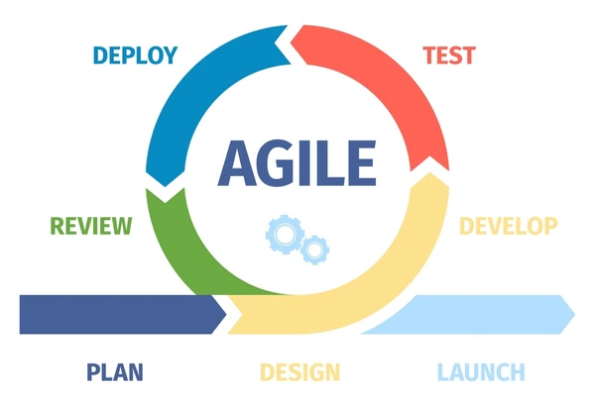
\includegraphics[width=1\textwidth]{figures/agile.png}
      \label{fig:1.6.0}
      \caption{The Agile Software Development Module}
\end{figure}

\subsubsection{Software required}
i.Microsoft Windows 10 Home or 11 Home\\ ii.Visual Studio Code for Windows \\
iii.Chrome, Firefox Web Browsers\\

\subsubsection{Frameworks and Libraries}
i.MongoDB Atlas for hosting our MongoDB database\\ ii.NodeJS to serve as the
runtime environment for our server\\ iii.ExpressJS as our web Framework\\
iv.HTML, CSS and JavaScript for our client side development.\\ v.Socket.io for
real-time bidirectional communication\\ vi.Git and GitHub for version control\\

\subsubsection{Hardware Requirements}
i.Processor (CPU):\\ Minimum: Intel Core i5-8th Gen or AMD Ryzen 5 3rd Gen (or
equivalent)\\ Recommended: Intel Core i7-10th Gen or AMD Ryzen 7 3rd Gen (or
equivalent)\\ ii.RAM: \\ Minimum: 8GB DDR4 RAM\\ Recommended: 16GB DDR4 RAM -
This would allow us to run multiple development tools smoothly\\ iii.Storage:\\
Minimum: 256GB SSD for faster loading times and overall performance\\

\subsection{Organization of Project}

The project is organized as follows: Chapter 1 covers the introduction, study
background, issue description, major and secondary objectives, significance of
the study, scope and limitations, process, and project organization. In Chapter
2, the literature review is discussed in order to offer an analysis of relevant
and current research studies. The project's methodology is thoroughly discussed
in Chapter 3. This is an extended version of the brief method from chapter 1.
Chapter 4 covers outcomes and analysis, or the evaluation and analysis of
results. Chapter 5 is meant to be the conclusion.\\ \newpage

\begin{center}
      \section*{CHAPTER TWO}
      \section{LITERATURE REVIEW}
\end{center}
\subsection{Overview}
This chapter conducts a comprehensive review of the existing literature
relevant to the field of study. It lays the foundation for the proposed project
by by providing a detail analysis of each of the projects parts. This chapter
explores the theoretical frameworks and methodological approaches used in
earlier studies. It offers an evaluation of of relevant projects pertaining to
WebRTC (Web Real Time Communication), SSR (Server Side Rendering), Scalable
Database management Systems and the use of ODM (Object Data Modelling)
libraries, Containerization, System architecture design to avoid SPOF (Single
Point of Failure) as well as Web Sockets. Reviews in this chapter are drawn
from online resources and journal publications.\\

\subsection{Current Issues of Concern}
The university system in Ghana is having a hard time keeping up with the
increasing number of students enrolled. The restricted housing options on and
around campus leads to bottlenecks, and students in remote locations frequently
do not have access to high-quality educational programs. Universities also find
it difficult to have a solid worldwide reputation and reach outside of Ghana.
These problems undermine both the overall influence of Ghanaian institutions
and educational equity. Furthermore, the increasing demand for flexible and
accessible learning options adds another layer of complexity. Students are
looking for educational options that work with their hectic schedules and
geographic constraints. This increasing demand for flexibility may not be met
by traditional classroom environments.\\

\subsection{Definition of Related Areas}
This section reviews detailed definitions that are closely related to the
project topic and scope, aiming to make things clearer and further
understanding of the project.\\

\subsubsection{WebRTC (Web Real Time Communication)}
WebRTC, which stands for Web Real-Time Communication, empowers peer-to-peer
associations without the require for third-party servers.Information sharing
over WebRTC is straightforward, supported by WebRTC APIs, and accessible at
many stages thanks to its simplicity. At first, servers are required for
clients to set up associations. After the initial setup, clients can talk
directly to each other, without the server involved.When a client sends data to
the signaling server, the server transfers this data to the other client. After
accepting this information, the client stores it locally. In this way, this
client sends its claim information to the server, which transfers it to the
other client. This trade guarantees both clients are mindful of each other,
encouraging an association foundation. Signaling servers, utilized for this
information trade, are standard servers with the sole reason of encouraging
client information trade.\cite{emmanuel2022design} The method of exchanging
information from one client to another in WebRTC is called signaling. In WebRTC
session establishment, the initial step is offer generation. A client
initiating communication creates an offer, typically a JavaScript object
encapsulating Session Description Protocol (SDP) data. The Session Description
Protocol (SDP) embedded within the offer specifies media capabilities, such as
video and audio codecs supported. The client sends this offer to the signaling
server, which forwards it to the other client. Upon receiving the offer, the
other client stores it locally and constructs an answer containing its own SDP
information. This answer, also transmitted via the signaling server, details
the recipient's media capabilities. While both parties now possess a mutual
understanding of each other's media offerings, an additional exchange of data,
termed ICE (Interactivity Connection Establishment) candidates, is necessary to
establish the peer-to-peer connection. Clients give URLs of these servers to
the WebRTC API to get ICE candidates. As the client makes an offer, ICE
candidates are recovered from the servers. These candidates are at that point
sent to the other client by means of the signaling server. The same handle
happens when creating answers. Once both clients have each other's SDP
information and ICE candidates, they can build up a coordinate peer-to-peer
association. Information transmission through WebRTC APIs from that point
happens straightforward between the clients, empowering efficient and secure
real-time communication.\\

\subsubsection{Web Sockets}
Web Sockets allow for two way communication, between a client like a web
browser and a server through a persistent, full-duplex connection. Unlike HTTP
requests where the client typically initiates communication and the connection
closes after each response, Web Sockets remain open, allowing both the client
and server to exchange messages at any time. This back and forth communication
is ideal for applications requiring low latency real time updates, such as chat
platforms, online games or collaborative editing tools. By using a handshake
process HTTP upgrade request and Web Socket Handshake to establish connections,
Web Sockets can efficiently receive data in both directions without the need
for repeated setup. This efficiency makes Web Sockets more effective for real
time communication compared to methods like polling or long polling. In summary
Web Sockets offer a solution, for creating web applications that demand
immediate responsiveness and minimal delays.\\

\subsubsection{Server Side Rendering}
Server-side rendering (SSR) is a procedure that renders a web page on the
server instead of within the browser. When a website is rendered on the server,
a completely rendered page is sent to the client and the client's JavaScript
bundle locks in and empowers the Single Page Application system to function.
Server side rendering (SSR) is a method employed in web development where the
server dynamically creates the HTML content of a web-page and sends it to the
clients browser. This differs from client side rendering, where the browser
uses JavaScript to generate the HTML content after receiving HTML from the
server.In SSR, when a user asks for a web page, the server handles the request,
collects the data from a database or external APIs, and then generates the HTML
content incorporating this data. The entire HTML page is then transmitted to
the client's browser for display without any processing. This approach can lead
to quicker initial page loading times. Improved search engine optimization
(SEO) since search engines can easily scan and index the HTML content. SSR is
frequently utilized in web applications developed with server side technologies
like Node.js, Django, Ruby on Rails and PHP. It proves advantageous for
websites with content or dynamically generated content where SEO and
performance play vital roles. Nonetheless implementing SSR may add complexity
to development and up keep efforts as it necessitates handling of server side
and client side logic to ensure consistency and optimal performance, across
platforms and devices.\\

\subsubsection{Success of  e-learning  platforms}
The rise of online learning platforms can be explained by several key factors.
First, their on-demand access model grants learners anytime, anywhere learning,
enabling them to progress at their own pace. Second, eLearning platforms offer
a varied content library, catering to various learning preferences through
multimedia elements like quizzes, interactive videos, and simulations. These
elements promote increased learner engagement and improve knowledge retention.
Finally, the inherent scalability and adaptability of eLearning platforms allow
them to effectively serve a wide range of learners with diverse learning needs.
Research conduction by S.Kim et al(2015)\cite{kim2023better} suggests that five
core principles significantly contribute to the success of an eLearning
platform:\\

\begin{enumerate}
      \item System Quality: This encompasses the platform's technical functionality,
            reliability, and user-friendliness. Here, factors like intuitive interface
            design, responsiveness, and seamless content delivery are crucial.\\
      \item Content Quality: This refers to the quality, relevance, and accessibility of
            learning materials hosted on the platform. Content should be well-organized,
            current, and aligned with established learning objectives.\\
      \item Instructional Design: This focuses on the effectiveness of the instructional
            methods employed in delivering the learning content. This includes factors like
            clear learning objectives, well-structured content delivery, and the use of
            appropriate pedagogical approaches.\\
      \item Online Interaction: This emphasizes the level of engagement and interaction
            within the platform. This includes fostering communication and collaboration
            among learners, instructors, and the learning materials themselves through
            discussion forums, group activities, and interactive assessments.\\
      \item Learning Outcomes Assessment: This refers to the process of measuring and
            evaluating the knowledge and skills acquired by learners against predefined
            learning objectives and performance standards. Effective assessment strategies
            should be integrated within the platform to track learner progress and provide
            feedback for continuous improvement.\\

            By focusing on these core principles, eLearning platforms can create an
            integrated and learner-centric teaching and learning environment.
\end{enumerate}

\subsubsection{Scalable No-SQL Database Management Systems}
MongoDB stands out as a liked No-SQL database recognized for its ability to
scale effectively. Its distributed architecture is the key, to this scalability
allowing it to manage data volumes and heavy traffic loads efficiently. MongoDB
utilizes sharing to distribute data among servers facilitating scaling. This
implies that as data and traffic increase you can expand the number of servers
in the MongoDB cluster to accommodate the growing demand. The adaptability of
MongoDB schema also plays a role in its scalability. Unlike databases MongoDB
does not mandate a predefined schema making it simple to introduce new fields
or modify existing ones without any downtime. This adaptability proves
beneficial in environments where requirements are subject to frequent changes.
Apart from scaling MongoDB also supports scaling by enabling you to enhance
individual server resources (such as CPU and RAM) within the cluster to manage
higher workloads. The combination of vertical scaling capabilities makes
MongoDB a scalable database solution suitable for various applications ranging
from small startups, to large enterprises.\\

\subsubsection{Containerization with Docker }
Docker, an example of containerization transforms the landscape of software
development and deployment by packaging applications and their requirements,
into self contained units known as containers. These containers operate
reliably across settings spanning from development, to production guaranteeing
behavior of applications regardless of their deployment location.
Containerization offers application segregation, flexibility and optimized
resource usage simplifying the development and deployment workflow while
enhancing resource efficiency compared to machines.\\

\subsubsection{System Architecture Design avoiding Single Point of Failure}
A critical aspect of system architecture design is the elimination or
mitigation of Single Points of Failure (SPOFs). An SPOF is a single component
whose failure can cause the entire system to become inoperable. It's really
important to make sure that a our system doesn't rely on one part that could
cause the whole thing to fail. When a single point of failure occurs it means
that if one component breaks the entire system will stop working. To prevent
this, methods like having backups and being able to handle faults are used to
keep the system running even if something goes wrong with one or more parts.
This is particularly crucial, in systems where any downtime could lead to
losses or affect how users interact with it. Ultimately avoiding points of
failure helps boost the reliability, availability and resilience of a system.\\

\newpage
\subsection{REVIEW OF RELATED AREAS}
This section provides an overview of other studies done by other authors that
are relevant to this work. It briefly outlines the working of the systems
examined in these related works, along with the methodologies used by the
respective authors. Furthermore, it evaluates the strengths and weaknesses in
these related works.\\

\subsubsection{1 Reviewed Work One}
\large\textbf{Review of Moodle LMS}\\

This review of Moodle explores the existing research and academic discourse
surrounding its development, implementation, and impact in educational
settings. This review typically examines various aspects such as its
effectiveness as a learning management system (LMS), pedagogical benefits,
challenges, and user perceptions.\\

\textbf{1.Effectiveness as an LMS}\\
Moodle is widely recognized for its flexibility and customization options, allowing educators to tailor the learning environment to specific needs (Al-Ajlan \& Zedan, 2008). Some Studies highlight its effectiveness in enhancing student engagement and interaction through forums, quizzes, and collaborative tools (Brandl, 2005). Other studies often show Moodle performing favorably against other LMS platforms in terms of user satisfaction and feature richness (Machado \& Tao, 2007).\\

\textbf{2.Pedagogical Benefits}\\
Dougiamas suggests Moodle enables active learning, collaboration, and self-paced study. The platform's tools, such as workshops and wikis, facilitate peer assessment and collaborative learning, fostering a deeper understanding of course material and the integration of  multimedia resources and interactive activities in Moodle courses has been shown to improve knowledge retention and comprehension.\\

\textbf{3.User perceptions and Experiences}\\
Students generally report a positive experience with Moodle, appreciating its accessibility and the ability to review materials at their own pace. Also being able to submit assignments, partake in quizzes and live discussions. However, continuous professional development and support are crucial for maximaizing the platform’s potential and ensuring effective usage. (Ullman \& Rabinowitz 2021).\\

\textbf{4.Challenges and Limitations}\\
Currently, Moodle primarily supplements traditional face-to-face classroom pedagogical methods. However, the imperative to transition fully to remote learning is increasingly critical. It's essential to define the learning context within the institution based on the capabilities and functionalities that the platform offers. This shift necessitates leveraging Moodle beyond its current supportive role to establish a comprehensive framework for remote education, addressing both technical and pedagogical challenges to enhance the institution's educational delivery and adaptability to modern learning environments.\\

\subsubsection{ Reviewed work two}
\large\textbf{The Process of Designing the Functionalities of an Online Learning Platform- A Case Study By; (Robert Oliwa, 2021)}\\

In this study, the author is looking into the process of designing the
functionalities of an online learning platform as proposed by three distinct
user groups: students, academics, and administrative staff. Furthermore, the
study aims to acquire insight into how these participants' opinions influence
the platform construction process. Using a case study design, the author
investigates whether users of the online learning platform can help define its
functionalities, specifically remote class creation and sharing, test
administration, and enhanced student activity reporting. Within the context of
Ghana Communications Technology University, by involving students, instructors,
and administrative staff in platform development, the proposed e-learning
platform for GCTU can address diverse needs and preferences, ensuring
accessibility, flexibility, and cost-effectiveness.\cite{oliwa2021process} \\

\textbf{Methodology}\\
The study used a mixed-methods approach to assess the design and functionality of an online learning platform through the eyes of students, professors, and administrative staff.\\

\textbf{Qualitative Data Collection}\\
Individual interviews were held with randomly selected individuals from each user group (students, teachers, and administrative personnel). These interviews provided detailed insights into participants' preferences, experiences, and needs for the online learning platform. Questions that were open-ended allowed participants to freely express their ideas and suggestions, leading to an even more specific understanding of their perspectives.\\

\textbf{Quantitative Data Collection}\\
A detailed online survey was distributed to a handful of students and teachers to get quantitative data on their thoughts and experiences with the online learning platform's functions or what said functions should be. The survey used structured questions and Likert scales to quantitatively assess participants' attitudes and preferences. This enabled a systematic examination of replies and the discovery of trends and patterns across various user groups. This study has established grounds for the development of a successful e-learning platform by employing a mixed-methods approach.\\

\textbf{Strengths of study}\\
1.By combining qualitative feedback from individual interviews with quantitative data from surveys, the study gathered a wide spectrum of viewpoints from students, teachers, and administrative personnel. \\
2.The integration of qualitative and quantitative data enabled a comprehensive synthesis of findings, resulting in useful suggestions for improving the design and effectiveness of an online educational platform.\\

\textbf{Limitations of the study}
1.The study sample size which was used might have been limited which would mean that the conclusions drawn from the study cannot be applicable in a more generalized setting or outside the context of the research.

\subsubsection{ Reviewed Work 3}
\large\textbf{Design And Implementation Of A Desktop Based System To Enhance Teaching Using Screen Sharing Technology Through Wlan Using GCTU As A Case Study( Adabogo Emmanuel,  Gertrude Fafali, 2022)}\\

This study aims to address several key challenges and to improve the overall
learning experience for both lecturers and students. Their approach aimed to
allow for seamless sharing of educational materials, presentations to eliminate
the need for costly subscription-based virtual classrooms. Using real-time
video and audio sharing mechanisms with WebRTC, they aimed to optimize the
platform to allow for interactive discussions and collaborations between
lecturers.\cite{emmanuel2022design}\\

\textbf{Methodology}\\
The methodology that the authors employed encompasses several key components aimed at designing and implementing a screen-sharing software for e-learning purposes.\\

\begin{enumerate}
      \item Technology Selection: The study begins by carefully identifying appropriate
            technologies for designing and implementing the screen-sharing system. This
            phase considers factors like efficiency, tolerance for errors, scalability, and
            cost efficiency.\\
      \item WebRTC Implementation: They utilize WebRTC to facilitate real-time
            communication and data transfer between lecturers and students. This technology
            provides a framework for audio and video peer to peer streaming over the web
            without the need for a third party, making it ideal for this application.\\
      \item Back-end Development: The utilized JavaScript runtime, NodeJS for the back-end
            development, which is responsible for the server-side operations.\\
      \item User interface design: They used HTML and CSS from the front-end or user
            interface, which is the part of the application that users interact with.\\
      \item Scalability Assessment: The system's scalability is assessed, taking into
            account elements such as the number of concurrent users it can support and its
            ability to handle increasing workload demands.\\
\end{enumerate}

\textbf{Strengths }\\
\begin{enumerate}
      \item By utilizing WebRTC technology and implementing real-time screen sharing
            capabilities, the study offers an innovative solution to address the challenges
            faced in traditional e-learning environments.\\
      \item The research's focus on building a desktop-based system with open-source
            technologies such as JavaScript, HTML, and CSS shows its focus on
            cost-effectiveness. The study offers universities a more financially
            sustainable alternative to pricey subscription-based virtual classroom
            applications.\\
      \item Along with basic screen-sharing capabilities, the system supports chat,
            file-sharing, and audio streaming. These extra features improve the e-learning
            experience by encouraging interaction and collaboration between lecturers and
            students in virtual classroom environments.\\
      \item The system's design prioritizes scalability, with up to 26 individuals using a
            single 4G WIFI interface. This scalability means that the system can
            effectively serve different class sizes while also adapting to the changing
            needs of educational institutions throughout time.\\
\end{enumerate}

\textbf{Limitations }\\
\begin{enumerate}
      \item The study focuses primarily on the development and testing of a screen-sharing
            system that employs WebRTC technology. It may not include all aspects of
            e-learning, including assessment methodologies, curriculum design, and learner
            engagement strategies.\\
      \item While the system has effective screen-sharing features, it may have technical
            restrictions such as bandwidth, latency, and device compatibility. Users with
            slower internet connections or older technology may have performance issues,
            which limit the system's accessibility and usability.\\
      \item The findings of the study may be specific to the context in which it was
            conducted, such as the particular technological infrastructure and user
            preferences within the university campus; drawing the results to other
            educational settings or cultural contexts might require additional change.\\
\end{enumerate}

\subsubsection{ Reviewed Work 4}
\large\textbf{Design and Implementation of Online-Learning platform with a large class size:
      Case study at University of Energy and Natural Resources-Ghana By; ( Peter
      Appiahene, Christopher Ninfaakang, 2017)}\\

This research explores the experimental use of a web-based platform to
supplement and improve the teaching and learning of the Computer Literacy and
Information Technology course at Ghana's University of Energy and Natural
Resources (UENR103). The study was conducted over two academic years with a
combined class of over 300 students each year. The document discusses the
methodology used in developing the online-learning platform, the results of
implementing the platform, student engagement through activities like group
discussions and self-assessment tests, and the overall response from students
and instructors to the technology-supported learning environment. The study
aims to showcase the application of online learning for large classes and how
it was implemented at the University of Energy and Natural Resources, providing
insights into the benefits and challenges of using technology in
education.\cite{appiahene2017design}\\

\textbf{Methodology }\\
The first phase of the study focused on developing a web-based
platform tailored to supplement the teaching and learning of the Computer
Literacy and Information Technology course at the University of Energy and
Natural Resources (UENR). This involved collaboration between instructional
designers, web developers, and subject matter experts to create a platform that
aligns with course objectives and student needs. The developed online-learning
platform was implemented over two academic years, accommodating a combined
class of over 300 students each year. This phase involved integrating the
platform into the course curriculum, providing access to students, and
facilitating instructor training on platform usage and management. Throughout
the study, student engagement was promoted through a variety of activities
supported by the online learning platform. These activities included group
discussions, self-evaluation assessments, interactive quizzes, multimedia
information delivery, and collaborative projects. The goal was to encourage
active learning, involvement, and knowledge retention among students.\\

\textbf{Strengths }\\
\begin{enumerate}
      \item Providing the option for students to read materials or watch videos caters to
            diverse learning styles and preferences, accommodating different ways in which
            students may absorb information effectively.\\
      \item The ability for students to submit assignments online and download materials
            from the platform streamlines the process of academic tasks, making it more
            convenient and efficient for both students and faculty.\\
      \item The implementation and testing phase of the project highlight the main features
            of the e-learning system, such as authentication mechanisms, database
            utilization, user account management, and error handling, indicating a
            comprehensive and well-thought-out development process.\\
\end{enumerate}

\textbf{Limitations}\\
The authors faced challenges in gathering information and data from
users for an objective assessment of the proposed e-learning products was
challenging. Expected users were unwilling to provide input or gave vague
information, leading to uncertain results.\\

\subsection{SUMMARY OF RELATED WORKS}
The reviewed literature highlights various aspects of e-learning platforms,
each with its strengths and limitations. The first review of Moodle LMS
underscores its flexibility and customization, effective student engagement,
and positive user perceptions, despite challenges in fully transitioning to
remote learning. The second work, a case study on designing functionalities for
an online learning platform, emphasizes the value of user input in platform
development, with a mixed-methods approach revealing insights into user
preferences and the importance of accessibility and flexibility. The third
review discusses a desktop-based screen-sharing system using WebRTC,
highlighting its cost-effectiveness, real-time interaction capabilities, and
scalability, although it may face technical limitations and context-specific
challenges. Lastly, the fourth review examines an online learning platform for
large classes at the University of Energy and Natural Resources, showcasing its
benefits in enhancing student engagement through diverse activities, while
noting the difficulty in gathering comprehensive user feedback for objective
assessment. Together, these works provide a comprehensive understanding of the
design, implementation, and impact of various e-learning systems, emphasizing
the importance of user-centered design, technological adaptability, and
continuous improvement to address the evolving needs of educational
environments.\\

\subsection{IDENTIFED GAPS FROM THE RELATED WORKS}
From the weaknesses identified in the four reviewed works, the following gaps
were identified:\\

\begin{enumerate}
      \item Limited Remote Learning Capabilities: Although Moodle and other platforms
            provide robust support for blended learning, there is an insufficient focus on
            fully remote learning environments. The transition to comprehensive online
            learning is hindered by inadequate leveraging of existing tools and features to
            support remote education effectively.\\

      \item User Involvement in Design: While the case study on designing online learning
            platform functionalities emphasizes user input, many platforms still lack
            significant engagement from students, instructors, and administrative staff in
            the design process. This limits the platform's ability to fully meet the
            diverse needs of its users.\\

      \item Technical Limitations in Real-Time Interaction: The desktop-based
            screen-sharing system using WebRTC offers innovative solutions for e-learning,
            but it does not comprehensively address issues related to bandwidth, latency,
            and device compatibility. These technical limitations affect the overall
            accessibility and performance of the system.\\

      \item Scalability and Performance: The online learning platform for large classes at
            the University of Energy and Natural Resources demonstrates the challenges of
            scaling e-learning systems. There is a need for solutions that can handle
            larger class sizes without compromising performance, ensuring seamless access
            for all students.\\

      \item Comprehensive Feature Integration: Many existing e-learning platforms do not
            fully integrate essential features such as audio transmission, real-time video
            conferencing, and collaborative tools. This results in a fragmented learning
            experience that can impede effective communication and interaction among
            users.\\
\end{enumerate}

\subsection{CURRENT SETUP OF E-LEARNING PLATFORMS}
\begin{figure}[H]
      \centering
      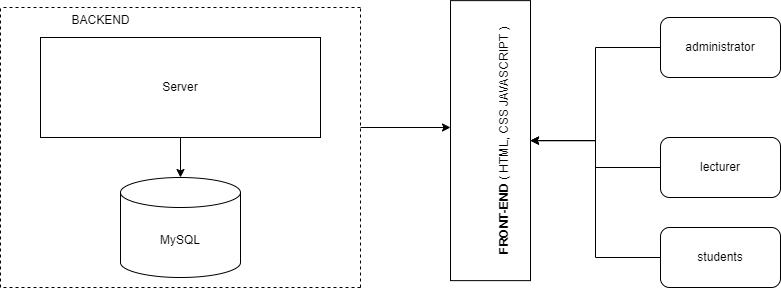
\includegraphics[width=1\textwidth]{figures/current.png}
      \caption{The current setup of e-learning systems (P. Appiahene et al, 2017)\cite{appiahene2017design}}
\end{figure}
The current setup of e-learning systems, as depicted in the provided diagram,
functions primarily as a drop box for resources, allowing users to access
content. Here's a detailed explanation:\\
\large\textbf{Backend}\\
\textbf{Server:} The server is the central component of the backend infrastructure. It
handles all the requests from the front-end and processes them. It is
responsible for managing the flow of data between the front-end and the
database.\\

\textbf{MySQL Database:} The MySQL database stores all the data related to the
e-learning system. This includes user information (administrators, lecturers,
students), course materials, assignments, and other educational resources. The
server interacts with the database to retrieve, store, and manage data.\\

\large\textbf{Front-End}\\
\textbf{Technologies Used:} The front-end of the system is built using HTML, CSS, and
JavaScript. These technologies are used to create the user interface that the
administrators, lecturers, and students interact with.\\

\large\textbf{User Roles}\\
\textbf{Administrator:} Administrators manage the overall system. They have access to
add, update, and delete resources, manage user accounts, and perform other
administrative tasks. They ensure that the system runs smoothly and
efficiently.\\

\textbf{Lecturer: }Lecturers can upload and manage course materials, assignments, and
other educational content. They interact with the system to provide resources
to students and possibly to receive assignments or tests from them.\\

\textbf{Students: }Students primarily use the system to access the educational content
uploaded by lecturers. They can download materials, view lectures, submit
assignments, and possibly take quizzes or exams if such features are
integrated.\\

\large\textbf{Functionality}\\
The current e-learning system setup is essentially a repository for educational
resources. It provides a centralized location where various users
(administrators, lecturers, and students) can interact with the system
according to their roles.\\

\textbf{Resource Upload and Management:} Lecturers and administrators can upload and
manage resources such as lecture notes, assignments, and multimedia content.\\
\textbf{Resource Access:} Students can access and download these resources, facilitating
their learning process.\\

\subsection{PROPOSED DESIGN OF E-LEARNING PLATFORM}
Our proposed e-learning solution is designed to provide a highly interactive
and efficient learning environment through the integration of advanced
technologies. At the core of our platform, we will leverage WebRTC to enable
real-time video conferencing, ensuring that live lectures and interactions are
smooth and responsive. For the back-end infrastructure, we will utilize the
Express web framework within the Node.js runtime, which will offer a scalable
and performant server-side solution. To manage and store data efficiently, we
will employ MongoDB, a NoSQL document-based database management system known
for its scalability and flexibility. This hybrid architecture is strategically
chosen to deliver a seamless performance and an optimal user experience across
a wide range of devices and varying network conditions, ensuring that our
e-learning platform is both robust and adaptable.\\

When selecting technologies for designing and implementing this system, it is
crucial to consider factors such as efficiency, fault tolerance, flexibility,
and reusability. Additionally, evaluating time and cost effectiveness,
user-friendliness, appealing interfaces, future maintenance needs, and overall
performance is essential.\\

\begin{figure}[H]
      \centering
      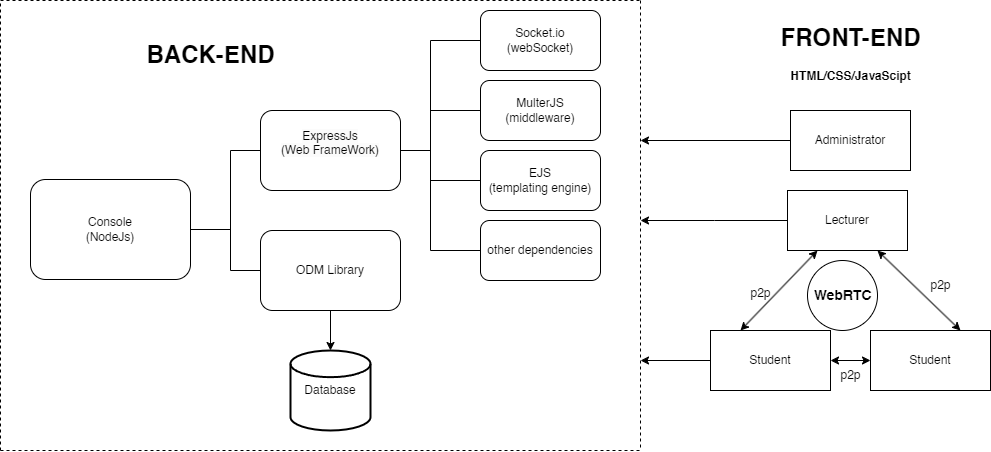
\includegraphics[width=1\textwidth]{figures/proposed.png}
      \caption{Our Porposed design of the E-learning platform (Solomon \& Avadzi 2024)}
\end{figure}

\subsection{CONCLUSION}
In conclusion, the literature review emphasises the important factors and
developments required for creating a successful e-learning platform. The
suggested solution claims to provide a robust, adaptable, and user-centric
educational experience by using WebRTC for real-time video conferencing, using
the Express framework on Node.js for the backend, and utilising MongoDB for
scalable data management. Emphasising elements like efficiency, fault
tolerance, and cost efficiency guarantees that the platform meets current
technological expectations while being adaptive to future improvements. This
complete strategy not only meets the immediate needs of smooth performance and
user engagement, but also positions the platform for long-term success and
growth in the ever-changing field of digital education.\\ \newpage

\begin{center}
      \section*{CHAPTER THREE}
      \section{METHODOLOGY}
\end{center}
\subsection{Overview}
This project is intended to use the Agile Software Development Methdology with
Scrum as the chosen framework. Agile emphasizes flexibility, iterative
development, as well as colaboration, making it ideal for projects that need to
adapt to changing requirements and foster continuous improvement. The Scrum
framework, a subset of Agile, is employed to structure the project’s
development process into a series of iterative cycles called Sprints. Each
Sprint includes stages of planning, development, testing and review. This
iterative process allows the team to deliver increments of the product
frequently, gather feednack, and adjust the course of development as needed.
The Agile approach with Scrum is particularly beneficial for projects where
requirements may evolve over time or where iterative feedback is crucial. Agile
methodologies like scrum are recommended for projects that require flexibility,
adaptability and continuous deleivery of functional increments.
\cite{schwaber2020scrum}\\

\subsection{Product Backlog Creation}
The Product Backlog is a crucial artifact in Scrum, representing a dynamic list
of work that needs to be done on the project. It includes everything from new
features and enhancements to bug fixes and technical debt. The management of
the backlog, involves prioritizing items based on their value to the project
and their alignment with the overall project goals. This prioritization is
essential for ensuring that the team is always working on the most important
tasks first. As the project evolves, so does the backlog, with items being
added, removed, or re-prioritized based on feedback and changing requirements.
\cite{schwaber2020scrum} \\ The product backlog for the e-learning platform
project is structured around a set of prioritized features and functionalities
designed to advance the research objectives of enhancing user engagement and
improving learning outcomes. Central to this backlog is the development of a
responsive user interface capable of adapting to a wide range of devices,
thereby ensuring accessibility and usability across different platforms. The
project also emphasizes the implementation of a content management system,
which is crucial for facilitating the seamless creation and management of
courses. Additionally, the integration of interactive components, such as a
video conferencing feature, is prioritized to actively engage students in the
learning process. Beyond these core functionalities, the backlog includes the
development of a secure user authentication system, which is essential for
protecting user data and maintaining the integrity of the platform. The
incorporation of real-time analytics is another key feature, enabling the
tracking of student progress and providing valuable insights that can be used
to tailor educational experiences. Furthermore, the support for multimedia
content is recognized as a critical element in enhancing the overall learning
experience, allowing for a richer and more varied educational environment. In
the figure below, we see how our product backlog is structured. This initial
list of items are at the “Epic Level” which means they are too big and vague
for us to be able to structure them based on technical infrastructure and other
dependencies. \\

\begin{figure}[H]
      \centering
      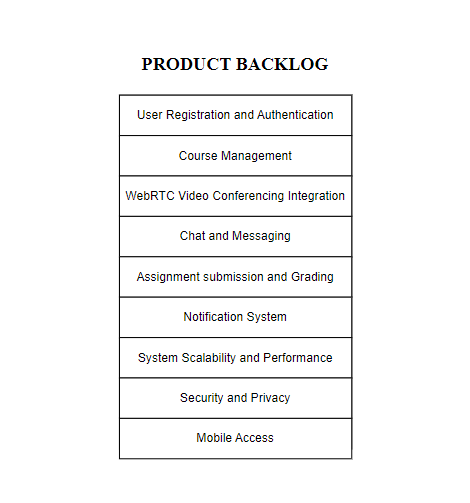
\includegraphics[width=1\textwidth]{figures/productbacklog.png}
      \caption{Product Backlog (Solomon \& Avadzi, 2024)}
\end{figure}

In the development of our Learning Management System (LMS), several key
features and functionalities are prioritized to enhance user experience and
system efficiency, which have made it into the product backlog. For User
Registration and Authentication, users need the capability to register for
accounts and log in securely to access their dashboards, while administrators
require tools to manage user roles and permissions to control access across the
LMS. In Course Management, administrators must be able to create, edit, and
delete courses, assign lecturers, and manage course schedules, while
instructors need to manage their assigned courses and students should be able
to register and enroll in courses to engage in the learning process. The
integration of WebRTC Video Conferencing is crucial, enabling instructors to
schedule and conduct live sessions, students to participate in these sessions,
and all users to share screens and record sessions for later access. The Chat
and Messaging system facilitates real-time communication, allowing students to
collaborate and instructors to send announcements. For Assignment Submission
and Grading, students need to submit their work online and instructors must
review and grade these submissions. The Notification System ensures users stay
informed about video sessions, deadlines, and announcements, with
administrators configuring settings to manage notification overload. System
Scalability and Performance are vital, requiring the ability to handle high
volumes of concurrent video sessions and optimize streaming quality based on
network conditions. Security and Privacy measures include implementing
encryption for video streams and enforcing data privacy policies. Lastly,
Mobile Access must be optimized to ensure that users can participate in courses
and video conferencing from various devices, with developers ensuring the LMS
is responsive and consistent across different screen sizes.\\

\subsection{Sprint Planning}
Sprint Planning is the event that kicks off each Sprint, where we selects items
from the top of the Product Backlog to work on during the upcoming Sprint. The
goal is to determine what can be delivered in the Sprint and how we will
accomplish that work. The outcome of Sprint Planning is a Sprint Goal, a clear
objective that the team commits to achieving, and a Sprint Backlog, which
includes the tasks required to meet that goal. This structured planning process
helps to ensure that the team is focused and aligned on what needs to be
accomplished within the Sprint
timeframe.\cite{beck2001agile}\cite{beedle2001agile}\cite{schwaber2020scrum}\\

In our upcoming sprint, we will focus on several crucial items from the product
backlog to drive our LMS project's progress. Our primary objective is to
enhance user registration and authentication processes, ensuring secure login
and comprehensive management of user roles and permissions by administrators.
We will also prioritize the development of robust course management features,
enabling administrators to create and manage courses, assign lecturers, and
establish schedules, while facilitating student registration and enrollment.
Integrating WebRTC video conferencing is essential, allowing instructors to
schedule and conduct live sessions, with features for screen sharing and
session recording. Additionally, we will implement chat and messaging
capabilities to support real-time communication and announcements. The sprint
will address assignment submission and grading workflows, streamline
notifications for users, and configure settings to prevent notification
overload. We will also focus on ensuring system scalability and optimizing
performance to handle concurrent video sessions and varying network conditions.
Security measures will include encryption for video streams and adherence to
data privacy policies. Finally, we will enhance mobile access to ensure a
consistent and responsive user experience across devices.\\

\begin{figure}[H]
      \centering
      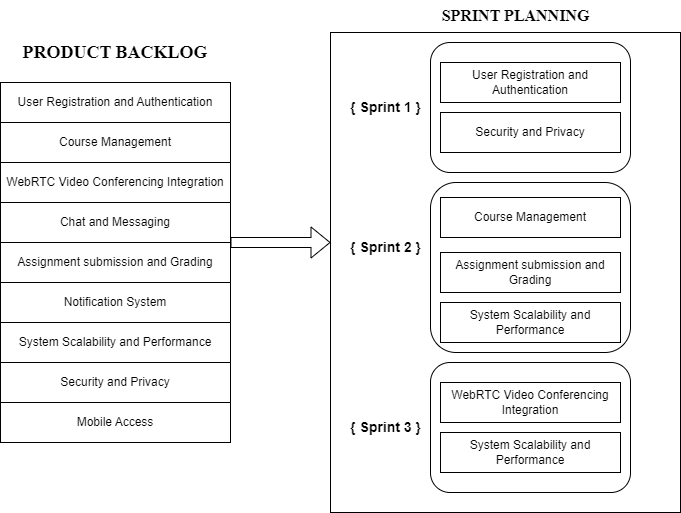
\includegraphics[width=1\textwidth]{figures/sprint-planning.png}
      \caption{Sprint Planning (Solomon \& Avadzi, 2024)}
\end{figure}

\subsection{Sprint Exxecution}
During Sprint Execution, the development team works on the tasks identified in
the Sprint Backlog to achieve the Sprint Goal. This phase is characterized by
intense collaboration among team members, who frequently communicate to ensure
progress is on track and to quickly address any issues that
arise.\cite{beck2001agile}\\ In this sprint execution phase, our focus will be
on systematically addressing the prioritized tasks from the product backlog to
ensure efficient delivery of key features. We will start by implementing and
testing enhancements to the user registration and authentication processes,
focusing on secure login and comprehensive management of user roles by
administrators. Next, we will develop and refine course management
functionalities, including the creation, editing, and scheduling of courses,
and enabling student enrollment. Concurrently, we will integrate WebRTC video
conferencing, enabling instructors to schedule live sessions, share screens,
and record sessions, while ensuring the feature supports smooth real-time
interaction for students. The chat and messaging system will be developed to
facilitate effective communication and announcements. We will also work on the
assignment submission and grading features to streamline the process for both
students and instructors. The notification system will be configured to provide
timely updates while avoiding overload, and performance optimizations will be
implemented to handle high volumes of concurrent sessions and varying network
conditions. Security measures will be integrated, focusing on encryption and
data privacy compliance. Finally, we will ensure the LMS is responsive and
functional on mobile devices, providing a consistent user experience. Regular
stand-ups and reviews will ensure progress tracking and address any issues
promptly, aligning with our sprint goals and timelines.

\subsubsection{Requirements}
The requirements of the project has been put into two parts. We have the
hardware requirements anad Software requirements. Hardware requirements refer
to the specific physical components and specifications needed for a computer
system or device to run a particular software application, perform a specific
function, or meet a certain level of performance. These requirements ensure
that the hardware is capable of supporting the software and tasks intended to
be executed on it. However it is advisable to have hardware that exceeds these
requirements for the optimal performance of services and
applications\cite{HANNIFIN201017}. On the other hand, the software requirements
refer to the technical specifications that explain the circumstances and
capabilities that a software system must have in order to perform properly
\cite{geeksforgeeks2024}. \clearpage \textbf{Hardware Requirements}\\

\begin{enumerate}
      \item Processor: 13th Gen Intel Core i7 13620 H
      \item RAM: 16GB DDR4 Random Access Memory (RAM)
      \item Storage: 256GB Solid State Drive (SSD)
      \item WebCam
      \item Microphone
      \item Router
\end{enumerate}

\textbf{Software Requirements}\\
The various software applications used in the design and implementation of the project includes:\\
\begin{enumerate}
      \item Operating System\\ The operating system provides the needed environment for
            software development and execution. For our project, we used Windows 11 Home.
            This is because it is compatible with a wide selection of development tools and
            applications, it offers enhanced performance and stability, the UI provides an
            intuitive and efficient workspace, which can improve productivity during
            development and testing phases. And because the scope of our project does not
            require enterprise-level features, Windows 11 Home offers a cost-effective
            solution without compromising on the essential functionalities needed for
            development.

      \item Web Browser\\ A web browser is a software application used to access
            information on the World Wide Web \cite{byjus2024}. For our project, Google
            Chrome was selected for its performance, developer tools, compatibility, and
            strong security features \cite{emmanuel2022design}, all of which contribute to
            a more efficient and effective development process.\\
      \item Text Editor\\ The text editor of choice is the Microsoft Visual Studio Code (VS
            Code). VS Code supports a wide range of programming languages and frameworks,
            making it suitable for diverse development tasks. It also has a rich ecosystem
            of extensions and plugins that enhance functionality, including support for
            debugging, code linting, version control, among others. It has an integrated
            terminal, it is cross-platform and has a user-friendly interface. \\

      \item MongoDB\\ MongoDB was chosen as our Database Management System (DBMS) for the
            project because of its flexibility and scalability. It is a NoSQL database that
            stores data in JSON-like format, allowing for dynamic schema design as well as
            the handling of unstructured or semi-structured data \cite{mongodb}. It is also
            well integrated in our programming language of choice, JavaScript.\\

      \item MongoDB Compass\\ MongoDB compass is a powerful Graphical user interfae ( GUI )
            for querying, aggregating and analysing your mongodb data in a visual
            environment. It allows users to connect to MongoDB deployment hosted on a
            remote server or on the users’ local machine. MongoDB compass provides
            real-time data and performance statistic visualisations, which allows us to
            better in understanding database behaviour and how to ways for query
            optimisation \cite{mongodb_compass}.\\

      \item JavaScript \& Node.js\\ Node.js is an important component of this project's
            technology stack, serving as a runtime environment for executing JavaScript
            code on the server. Node.js is based on Chrome's V8 JavaScript engine, which
            provides a non-blocking, event-driven architecture that is ideal for
            asynchronous processes and scalable network applications. It also provides a
            solid foundation for developing server-side apps and APIs, by leveraging the
            npm ecosystem to integrate a diverse set of libraries and modules that simplify
            development processes \cite{nodejs2024} \cite{geeksforgeeks2024}
            \cite{w3schools2024}.\\

      \item WebRTC \& PeerJS\\ PeerJS is used to simplify the project's implementation of
            peer-to-peer communication. PeerJS provides an easy-to-use API that
            encapsulates the difficulties of setting up WebRTC peer connections, allowing
            clients to exchange real-time audio, video, and data. It manages the signalling
            process, peer finding, and connection management, allowing developers to
            concentrate on application logic rather than underlying infrastructure.
            PeerJS's capabilities are critical for developing real-time communication
            features like video chat and file sharing without having to deal with the
            intricacies of WebRTC protocols \cite{webrtc2024} \cite{peerjs2024}.\\
            \begin{figure}[H]
                  \centering
                  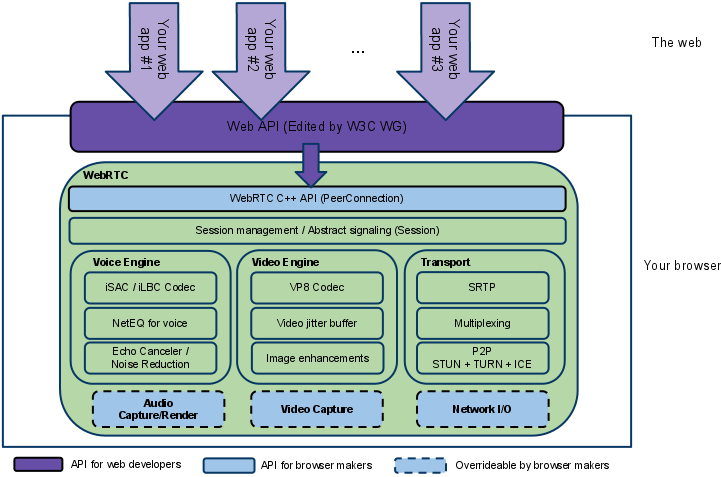
\includegraphics[width=1\textwidth]{figures/w3rtc.png}
                  \caption{WebRTC architecture  (W3C WG, 2022)}
            \end{figure}

      \item Embedded JavaScript (EJS)\\ EJS (Embedded JavaScript) is used to render HTML
            templates on the server side of and we will use this as our templating engine
            for rendering dynamic pages. EJS allows us to embed JavaScript code directly
            into HTML pages, making it easier to generate dynamic content based on
            server-side data. This templating engine supports template inheritance and
            partials, which make it easier to create reusable and maintainable HTML
            components. EJS works smoothly with Node.js applications, giving us an
            efficient way to render views and manage dynamic
            content\cite{geeksforgeeks2024ejs}.\\

      \item Cascading Style Sheets\\ CSS (Cascading Style Sheets) is used to specify the
            visual appearance and layout of the project's web pages. CSS separates content
            from design, allowing developers to apply consistent styling across various
            pages and components. CSS allows developers to customise the look and feel of
            their applications, including colour schemes, typography, spacing, and
            responsive design\cite{w3schools2024css}.\\
\end{enumerate}

\subsubsection{Design and Implementation}
The system architecture diagram provides a comprehensive overview of the LMS's
core components and their interactions, serving as a high-level abstraction to
facilitate understanding of the system's overall structure. At its core, the
diagram illustrates the main elements of the system: the user interface,
application server, WebRTC server, and database, detailing how these components
are interconnected and communicate with each other. The user interface
represents the front-end layer, where users interact with the system. It
includes all the elements that users see and interact with, such as dashboards,
course management tools, and video conferencing interfaces. This layer ensures
a seamless user experience and interfaces with the application server to handle
user requests and present data. The application server functions as the central
processing unit of the system. It manages business logic, handles user
requests, and facilitates communication between the user interface and the
database. It processes authentication, authorization, course management,
assignment submissions, and other critical operations, ensuring that the system
functions smoothly and efficiently. The WebRTC server is integral for real-time
communication, enabling live video sessions, screen sharing, and recording
functionalities. It supports the interactive aspects of the LMS, allowing
instructors and students to engage in real-time video conferencing and
collaborate effectively. The database component stores all persistent data,
including user information, course details, assignment submissions, and chat
messages. It interacts with the application server to retrieve and store data
as needed, ensuring data integrity and accessibility.\\

\begin{figure}[H]
      \centering
      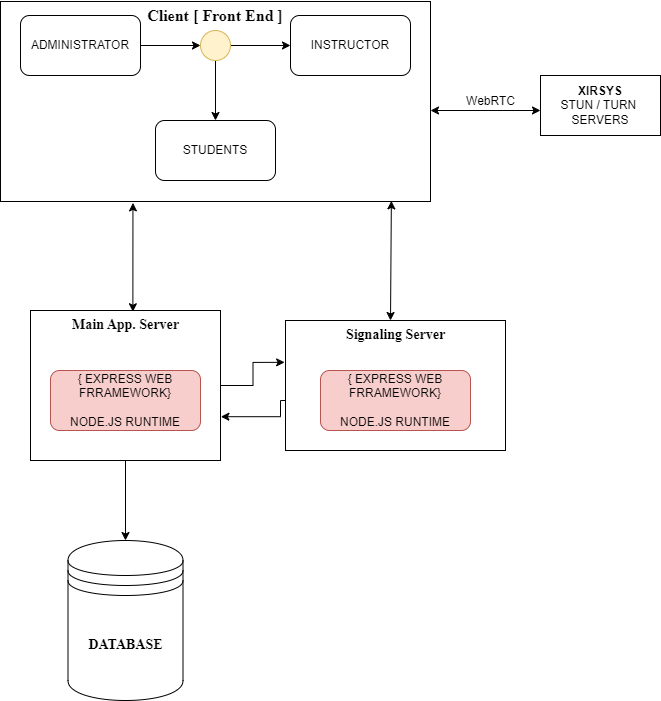
\includegraphics[width=1\textwidth]{figures/System Architecture.drawio.png}
      \caption{System Architecture (Solomon \& Avadzi, 2024)}
\end{figure}

\subsubsection{User Registration and Login}
The process begins when a user accesses the registration or login page of the
platform. The login process is straightforward. Users must input their user id
(student id for students, admin id for administrators and lecturer id for
lecturers ) and password. The system then checks these credentials against the
database to authenticate the user. If the details match, the user is redirected
to their dashboard, where they can access various features of the platform. In
the case of an authentication failure, an error message is displayed, prompting
the user to retry or recover their password.\\
\begin{figure}[H]
      \centering
      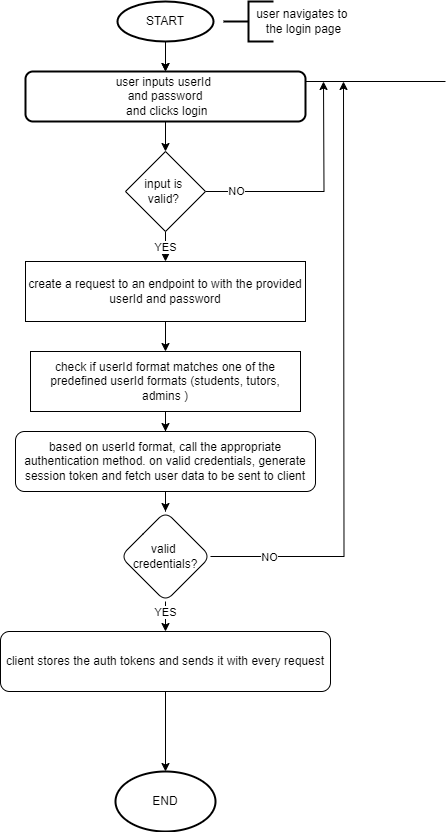
\includegraphics[width=1\textwidth]{figures/login flowchart.drawio.png}
      \caption{User Login Flow Chart (Solomon \& Avadzi, 2024)}
\end{figure}

\subsubsection{Video Conferencing Flow Chart}
Upon the initiation of a session, a participant’s identification and course
details are validated. This is facilitated through a structured URL pattern
that determines the user type (either lecturer or student) and redirects the
user to the appropriate meeting room. The participant's credentials and course
information are stored temporarily in the session storage to ensure continuity
across the session.Once the user accesses the meeting room, the system
retrieves the course and user information to ensure proper authentication and
authorization. Participants' data is then used to set up the communication
environment, where the information about the participants, such as user IDs and
their roles (e.g., lecturer or student), is crucial for managing permissions
and interactions during the session. The system establishes peer-to-peer
connections between participants using the WebRTC framework. This involves
setting up peer connections, exchanging session descriptions (SDP), and
handling ICE (Interactive Connectivity Establishment) candidates, which are
essential for establishing the media streams over varying network conditions.
The negotiation process, initiated either by the host or other participants,
involves creating and setting session descriptions, which detail the media
formats and parameters supported by each peer. \\
\begin{figure}[H]
      \centering
      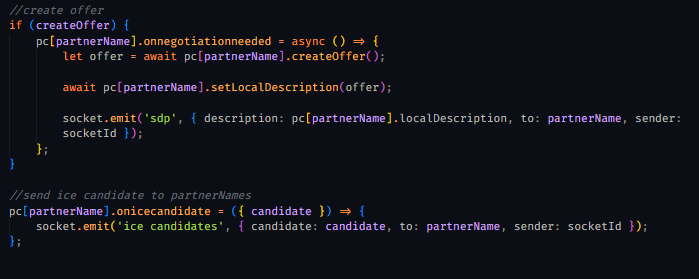
\includegraphics[width=1\textwidth]{figures/create-offer.png}
      \caption{JavaScript code to establishing connection (Solomon \& Avadzi, 2024)}
\end{figure}
This ensures compatibility and seamless media exchange. Participants' media streams, whether video or audio, are then captured and transmitted across these peer connections. The system ensures that each participant's media is rendered on the interfaces of other participants, allowing for real-time interaction. The handling of media streams is dynamic, enabling participants to toggle between different media sources, such as sharing their screens or switching between audio and video streams. This is particularly useful in a classroom setting, where a lecturer might need to present material via screen sharing.\\
Throughout the session, the system monitors the connection state and signaling state of each peer connection, ensuring that any disruptions, such as disconnections or failures, are managed promptly. The interface dynamically adjusts to reflect the current state of the connections, ensuring that participants are kept informed of any issues, such as a peer leaving the session. Additionally, the platform provides functionality for managing the session lifecycle, including the ability for the host (typically the lecturer) to terminate the session for all participants. This action is accompanied by an update of the course meeting information, which ensures that the session details are accurately recorded and that participants are appropriately redirected once the session ends.\\

\begin{figure}[H]
      \centering
      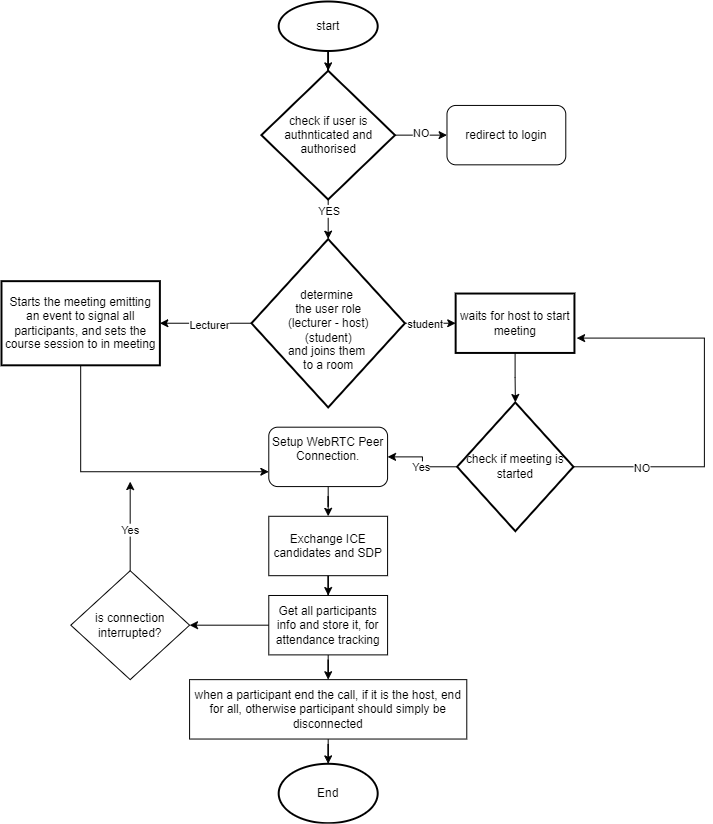
\includegraphics[width=1\textwidth]{figures/webrtc.drawio.png}
      \caption{High Level Video Conferencing Flow chart (Solomon \& Avadzi, 2024)}
\end{figure}

\subsubsection{Level 0 Data Flow Diagram (DFD) for Video Conferencing Feature}
The Level 0 Data Flow Diagram (DFD) provides an overview of the video
conferencing feature within the e-learning platform, illustrating the main
processes, data stores, and external entities involved. It serves as a
high-level representation that abstracts detailed internal processes,
emphasizing primary data flows and interactions.\\

\begin{itemize}
      \item Components:
            \begin{enumerate}
                  \item External Entities:\\ a. Lecturer: Initiates and participates in the RTC
                        session.\\ b. Student: Joins and participates in the RTC session.\\
                  \item Processes: \\ a. RTC API: Serves as the central process, coordinating the
                        initiation and participation in RTC sessions.\\ b. User Authentication: Ensures
                        that the user (lecturer or student) is authenticated before accessing the RTC
                        API.\\ c. Signaling Server: Establishes and manages the WebRTC connection
                        between participants.\\
                  \item Data Stores:\\ a. Data: Repository for storing session data, such as attendance
                        tracking and session metadata.\\
            \end{enumerate}
      \item Data Flows:
            \begin{enumerate}
                  \item 1.Initiates RTC Session: The lecturer initiates a Real-Time Communication (RTC) session by sending a request to the RTC API along with their lecturerId.\\
                  \item Join RTC Session: Students join the RTC session by sending a request to the RTC
                        API along with their studentId.\\
                  \item User Information: The RTC API forwards user information to the User
                        Authentication process to authenticate the user.\\
                  \item Authenticate User: User Authentication validates the user credentials and sends
                        an authentication status back to the RTC API.\\
                  \item Setup WebRTC Connection: The RTC API interacts with the Signaling Server to
                        establish the WebRTC connection.\\
                  \item Attendance Tracking: The Signaling Server sends session data, including
                        attendance tracking, to the Data store.\\
            \end{enumerate}
\end{itemize}

\begin{figure}[H]
      \centering
      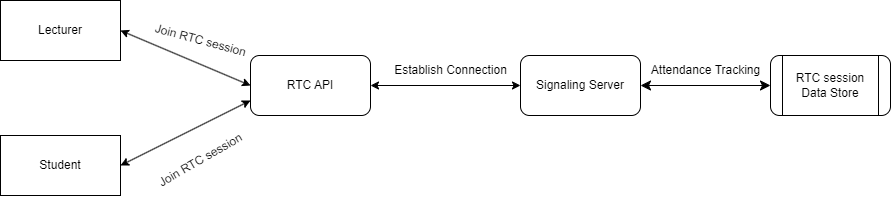
\includegraphics[width=1\textwidth]{figures/data-flow-level-0.drawio.png}
      \caption{Level 0 DFD for video conferencing (Solomon \& Avadzi, 2024)}
\end{figure}

\subsubsection{Level 1 Data Flow Diagram (DFD) for Video Conferencing Feature}
The Level 1 Data Flow Diagram (DFD) delves deeper into the internal processes
of the video conferencing feature, detailing the specific functions within the
RTC API and Signaling Server processes. It provides a more granular view of
data interactions and flow within the system.\\

\begin{itemize}
      \item Components
            \begin{enumerate}
                  \item External Entities: \\
                        a. Lecturer: Continues to initiate and participate in RTC
                        sessions. \\
                        b. Student: Continues to join and participate in RTC sessions.\\
                  \item Processes: \\
                        a. RTC API: Further decomposed into functions handling session
                        initiation, management, and participation. \\
                        b. Signaling Server: Manages the signaling and connection establishment for WebRTC, along with attendance
                        tracking.\\
                  \item Data Stores:\\
                        a. RTC Session Data Store: Stores detailed session data, including
                        connection logs, attendance records, and session metadata.\\
            \end{enumerate}
      \item Data Flows:
            \begin{enumerate}
                  \item Initiates RTC Session: The lecturer sends a request to the RTC API to initiate an RTC session, containing the lecturerId.\\
                  \item Join RTC Session: Students send requests to the RTC API to join the RTC session, containing their studentId.\\
                  \item Establish Connection: The RTC API processes the session initiation and participation requests, then interacts with the Signaling Server to establish the WebRTC connection.\\
                  \item Attendance Tracking: The Signaling Server tracks attendance and sends detailed session data to the RTC Session Data Store for storage and later retrieval.\\
            \end{enumerate}
      \item Detailed Process Descriptions:\\
            \begin{enumerate}
                  \item RTC API:\\
                        a. Session Management: Handles the initiation and management of RTC sessions, ensuring that requests from lecturers and students are processed appropriately.\\
                        b. Connection Coordination: Coordinates with the Signaling Server to establish and manage WebRTC connections.\\
                  \item Signaling Server:\\
                        a. Connection Establishment: Manages the signaling process required to establish WebRTC connections between participants.\\
                        b. Attendance Tracking: Monitors and records attendance, sending this data to the RTC Session Data Store for persistent storage.\\
            \end{enumerate}
\end{itemize}

\begin{figure}[H]
      \centering
      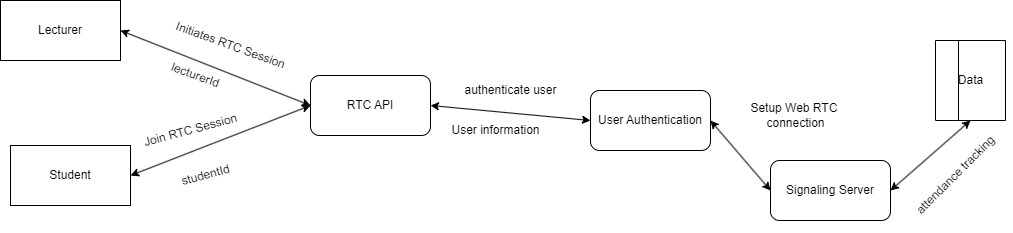
\includegraphics[width=1\textwidth]{figures/dataflow-level1.drawio.png}
      \caption{Level 1 DFD for Video Conferencing Platform (Solomon \& Avadzi, 2024)}
\end{figure}

The Level 0 and Level 1 Data Flow Diagrams for the video conferencing feature in the e-learning platform provide a structured and detailed view of the system's data interactions. These diagrams help in understanding the primary processes involved, the flow of data between them, and the interactions with external entities. The level of detail provided in Level 1 further clarifies the internal workings of the RTC API and Signaling Server, ensuring a comprehensive understanding of the video conferencing feature's operation.\\

\subsubsection{Entity Relationship Overview for the Video Conferencing feature}
The Entity-Relationship Diagram (ERD) illustrates the data structure of the video conferencing feature within the e-learning platform. It showcases the various entities involved, their attributes, and the relationships between them. This ERD is pivotal for understanding how the system manages courses, submissions, and real-time communication (RTC) sessions.\\

\begin{figure}[H]
      \centering
      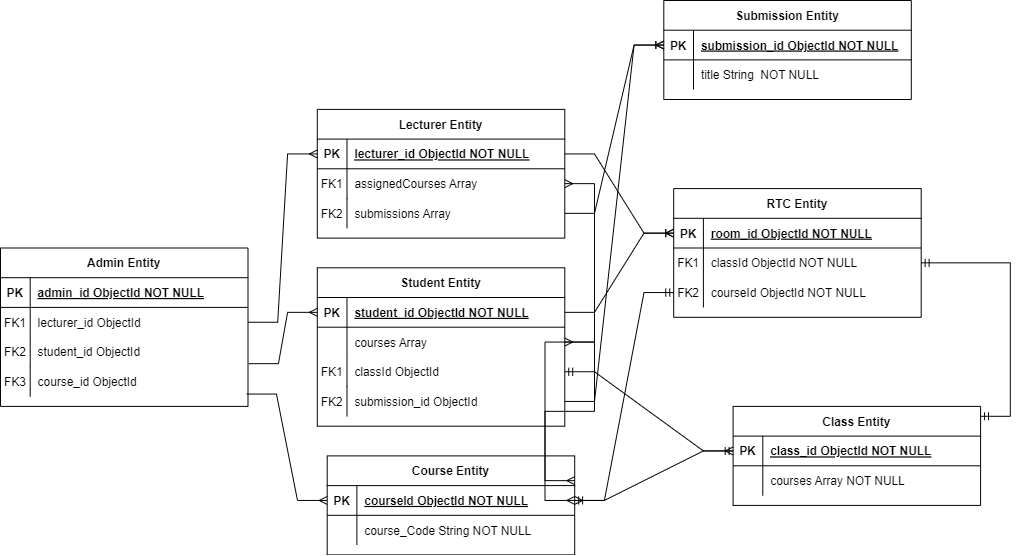
\includegraphics[width=1\textwidth]{figures/entity-relationship diagram.drawio.png}
      \caption{Entity Relationship Diagram for the Video Conferencing (Solomon \& Avadzi, 2024)}
\end{figure}
The Admin Entity is the administrative core of the system, uniquely identified by the adminid attribute. It maintains references to lecturers, students, and courses through foreign keys, ensuring streamlined management of these entities. The Lecturer Entity, identified by lecturerid, includes arrays for assigned Courses and submissions, reflecting the courses they manage and the submissions they oversee. Similarly, the Student Entity, identified by studentid, contains arrays for courses and a foreign key for classId, linking students to their classes and courses. The Course Entity, with courseId as its primary key, holds vital information about each course, including a unique course code and a reference to the associated class. The Class Entity aggregates courses through an array, highlighting the collective structure of classes within the platform. The RTC Entity, identified by roomid, is crucial for real-time communication, linking each RTC session to specific classes and courses, thereby facilitating seamless virtual interactions. The Course Entity, with courseId as its primary key, holds vital information about each course, including a unique course code and a reference to the associated class. The Class Entity aggregates courses through an array, highlighting the collective structure of classes within the platform.  The RTC Entity, identified by roomid, is crucial for real-time communication, linking each RTC session to specific classes and courses, thereby facilitating seamless virtual interactions.\\

\subsubsection{Course Management and Submission Management}
Upon successful login, students and lecturers access the course management area, which provides a tailored list of courses based on the user’s level, program, and faculty. For students, the registration process involves using system-generated registration codes to enroll in courses. Once registered, the courses are added to the student's courses , effectively integrating the student into the course structure. Lecturers, on the other hand, are tasked with managing their assigned courses. This involves adding lessons and materials to course chapters and initiating live class sessions, thus centralizing course material management.

The submission management system is meticulously designed to streamline the creation and handling of assignments. Lecturers initiate this process by entering essential details such as the course code, title, instructions, and timelines. The system organizes these details into structured objects and links them to the appropriate course using the course code. If no existing submission record is found, a new entry is created in the Submissions collection. For existing records, the system employs the \$addToSet operator to append new submissions, ensuring no duplication. Students interact with this system to access and submit assignments. Upon submission, the system associates the uploaded files with the student’s record in the student-submissions field of the Submissions collection. This organized storage mechanism ensures easy retrieval and review. Post-submission, lecturers can review and grade the work, with the system updating each entry's status to indicate whether it has been graded. Additional functionalities, such as bulk download of submissions and robust error handling, enhance the platform’s utility, ensuring smooth interactions and efficient data management.\\
The ERD and the detailed workflows of course management and submission management provide a comprehensive blueprint of the e-learning platform’s data interactions. This structured approach ensures efficient management of academic activities, fostering seamless communication and collaboration between lecturers and students. The robust design facilitates effective course management, organized submission handling, and real-time communication, thereby enhancing the overall educational experience.\\

\subsubsection{Session Traversal Utilities for NAT (STUN)}
STUN, an IETF protocol, supports real-time communication such as phone, video, and messaging over IP networks. It provides a method to establish connections with users behind a Network Address Translation (NAT) firewall, which conceals their IP addresses within the local network (LAN). The process begins with the initiating party sending a request to the STUN server, which records the device's IP address (such as for video). Subsequently, using protocols like WebRTC or ICE, a peer-to-peer connection is established. Unlike application layer gateways (ALGs) that also enable two-way communication through NATs, STUN does not necessitate any router configuration\cite{emmanuel2022design}.\\

\subsection{Sprint Review and Retrospective}
The Sprint Review, held at the end of each Sprint, serves as a critical checkpoint to inspect the work completed and gather feedback from users. During this meeting, the development team demonstrates the completed work to the users, highlighting the deliverables achieved during the Sprint. The discussion focuses on comparing what was accomplished against the initial Sprint goals and planned tasks. This review is not merely a showcase of completed work but a dynamic forum where stakeholders can provide valuable input. This feedback can lead to necessary adjustments in the Product Backlog, ensuring that the project remains aligned with users’ expectations and evolving requirements. Following the Sprint Review, the team engages in a Sprint Retrospective. This meeting is dedicated to reflecting on the Sprint's processes and outcomes. The Retrospective provides an opportunity for the team to candidly discuss what went well, what did not go as planned, and what could be improved in future Sprints. The team identifies specific areas for improvement, such as workflow optimizations, communication enhancements, or technical practices that need refinement\cite{schwaber2020scrum}.\\

Within the context of our project, these meetings are essential for several reasons. The Sprint Review allows us to ensure that the development of the video conferencing feature and the overall e-learning platform meets the users’ needs. By demonstrating the functionality related to real-time communication, course management, and submission handling, we can obtain immediate feedback and make adjustments to the RTC API, signaling server, and other components as necessary.\\

The Sprint Retrospective, on the other hand, enables the team to reflect on the technical challenges encountered during the development of these features. For instance, we can discuss the integration of STUN for NAT traversal in our WebRTC implementation, the efficiency of our data flow for course and submission management, and any issues related to the entity-relationship mapping of our database. By evaluating these aspects, we can identify and implement changes that will enhance our development process, improve code quality, and ensure robust functionality in future Sprints. They ensure that the team remains responsive to user feedback, adapts to changes efficiently, and continuously seeks ways to enhance their effectiveness. These meetings contribute to the iterative and incremental development approach, which is crucial for delivering a high-quality e-learning platform that meets both current and future needs of users.

\subsection{Summary of Chapter}
This chapter describes how we used the Agile methodology to direct the development of the e-learning platform's video conferencing capability. Iterative development was used to build the project, integrating ongoing criticism and enhancements. A variety of software tools and technologies were used, with HTML and CSS being used for the user interface design and JavaScript serving as the main language for the backend. The server system was hosted on personal computers during the deployment process. For efficient real-time interactions, data transmission between devices was facilitated by the platform's communication, which depended on strong internet connections. Sprint Reviews and Retrospectives were held during the development process to assess the project's progress, get input, and apply improvements. This helped to guarantee that the project satisfied user requirements and upheld strict performance and security criteria.\\ \newpage

\begin{center}
      \section*{CHAPTER FOUR}
      \section{ANALYSIS AND RESULTS}
\end{center}

\subsection{Overview}
This chapter presents a comprehensive analysis and the resultant findings of the implemented video conferencing feature within the e-learning platform. It carefully looks into the system's overall efficiency, user input, and performance metrics. The chapter attempts to verify the system's scalability, dependability, and user satisfaction through thorough testing and assessment. To collect information, evaluate functionality, and pinpoint areas in need of development, a range of analytical techniques and instruments were utilised. The findings are presented in a methodical manner, offering insights into the effectiveness of the system's functioning, any bottlenecks, and how they affect the educational process. This chapter is an essential part of the study since it provides findings based on data and suggestions for improvements in the future.\\

\subsection{User Interface}
The user interface (UI) of the e-learning platform has been meticulously designed to cater to both students and lecturers as well as admins, ensuring a seamless experience across different user roles. Each page and interaction is crafted to enhance usability while supporting the educational process through intuitive navigation and access to essential features.\\

\subsubsection{Login Page}
The login page serves as the entry point to the platform for both students and lecturers as well as admins. It is designed with simplicity and security in mind. Users are prompted to enter their credentials, which are securely processed to grant access to the system. The page features a clean layout with clearly labeled input fields for the user id and password, as well as options for password recovery. The UI ensures that users can quickly log in and proceed to their respective dashboards, minimizing friction and enhancing the overall user experience.\\

\begin{figure}[H]
      \centering
      \includegraphics[width=1\textwidth]{figures/loginUi.png}
      \caption{Login Page UI (Solomon \& Avadzi, 2024)}
\end{figure}

\subsubsection{Students Courses Page}
Upon logging in, students are directed to their courses page, which serves as their primary hub for academic activities. This page displays a list of all the courses the student is enrolled in, presented in a visually organized manner. Each course entry includes key details such as the course title, instructor's name, and upcoming deadlines. The interface is designed to make navigation straightforward, with clickable course titles leading to the course view page. The UI also incorporates quick access to essential features such as assignments, discussion forums, and video conferencing sessions, ensuring that students can easily manage their coursework and participate in class activities.\\

\begin{figure}[H]
      \centering
      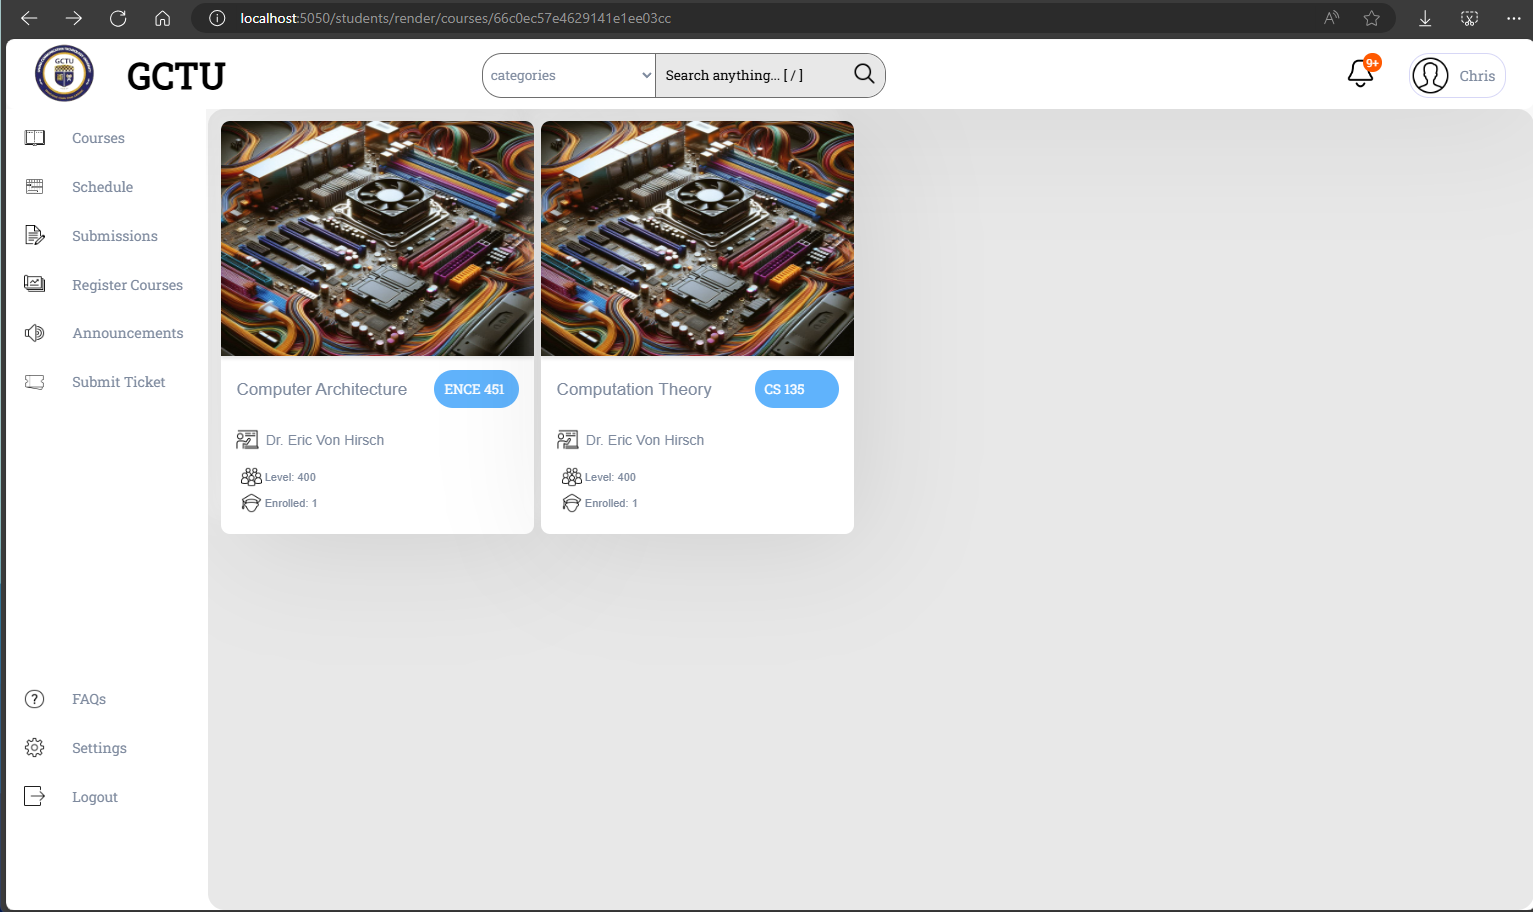
\includegraphics[width=1\textwidth]{figures/students-courses.png}
      \caption{Students list of Courses Page UI (Solomon \& Avadzi, 2024)}
\end{figure}

\subsubsection{Lecturers Courses Page}
Lecturers, upon logging in, are presented with their own courses page, which functions as a centralized dashboard for managing their teaching responsibilities. Similar to the students' page, this interface displays all the courses the lecturer is responsible for, along with relevant details such as scheduled class times and student enrollment numbers. The UI for lecturers includes additional functionalities like course creation and editing tools, assignment management, and access to student progress tracking. This interface is designed to streamline the administrative tasks associated with course management, allowing lecturers to focus more on delivering quality education.\\

\begin{figure}[H]
      \centering
      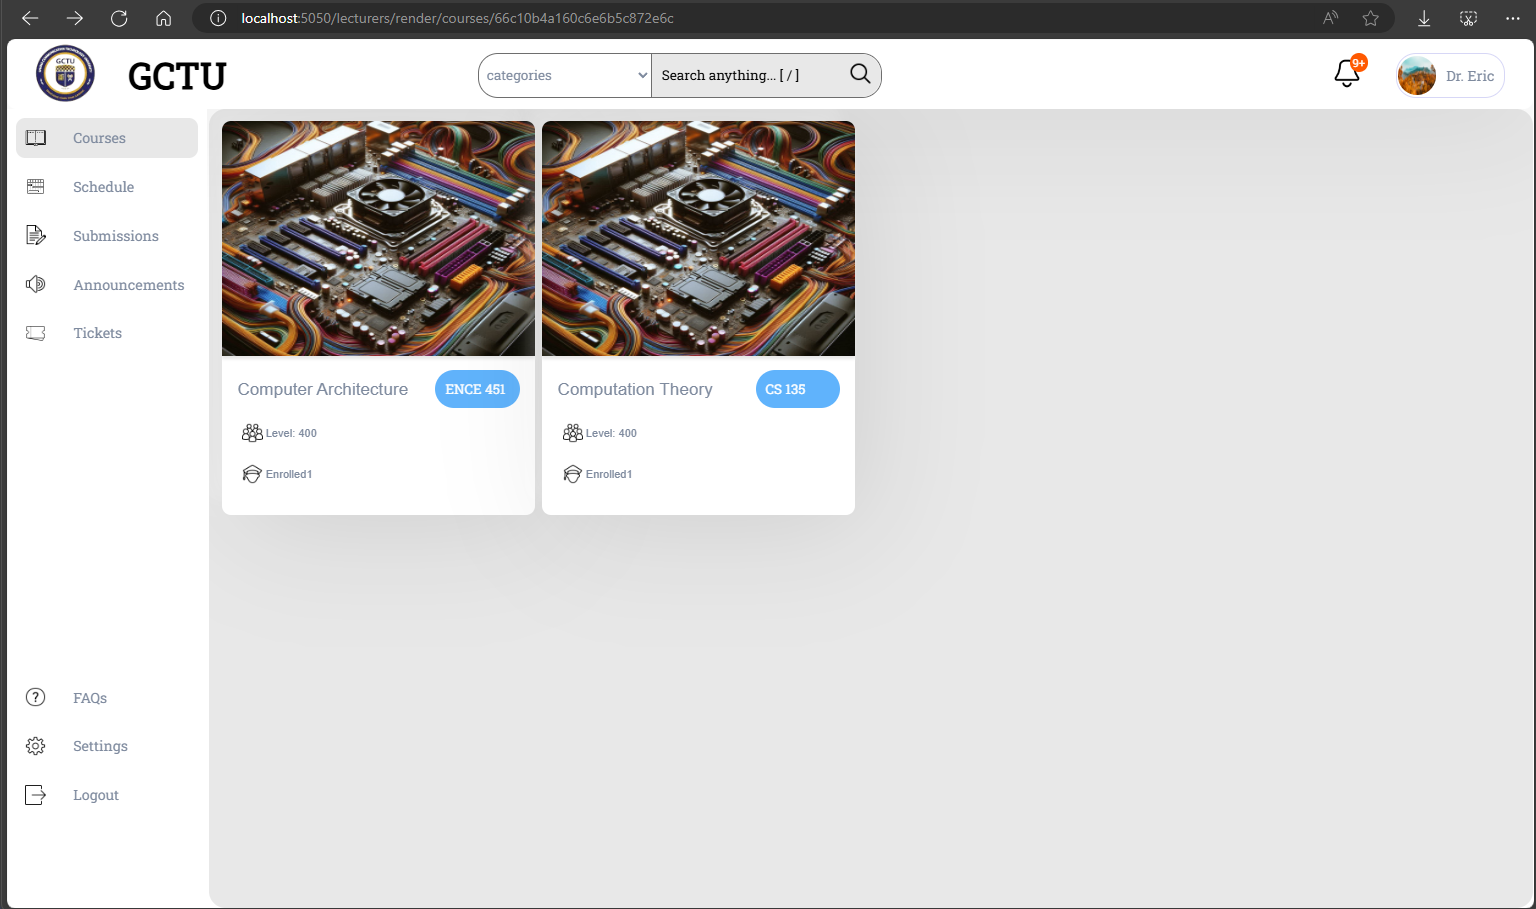
\includegraphics[width=1\textwidth]{figures/lecturers-courses.png}
      \caption{Lecturers List of courses Page UI (Solomon \& Avadzi, 2024)}
\end{figure}

\subsubsection{Course View Page (for Both Students and Lecturers)}
The course view page is a shared interface for both students and lecturers, tailored to provide each with the relevant tools and information they need. For students, this page offers access to all course materials, including lecture notes, videos, assignments, and discussion forums. The UI is designed to make content easily accessible, with clear categorization and navigation options. Lecturers, on the other hand, see additional options for uploading content, managing assignments, and monitoring student participation. This page is pivotal in facilitating the learning process, providing a structured environment where all course-related activities are centralized.\\

a.The Lecturer’s course details page\\
\begin{figure}[H]
      \centering
      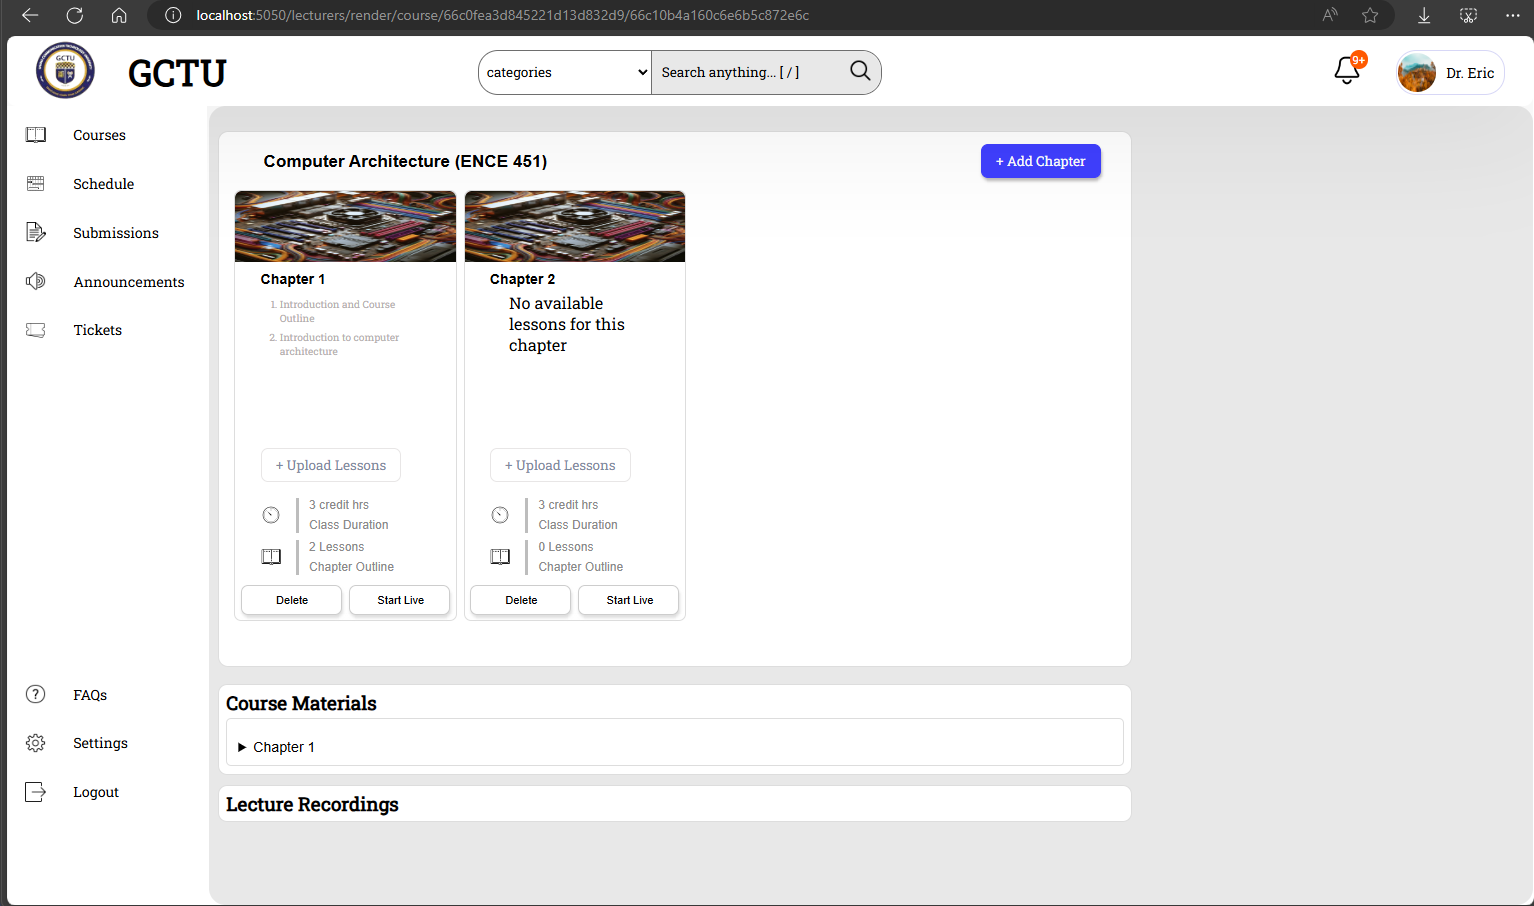
\includegraphics[width=1\textwidth]{figures/lect-c-dets.png}
      \caption{Lecturer Course View Page UI (Solomon \& Avadzi, 2024)}
\end{figure}

b.The Student’s  course details page\\
\begin{figure}[H]
      \centering
      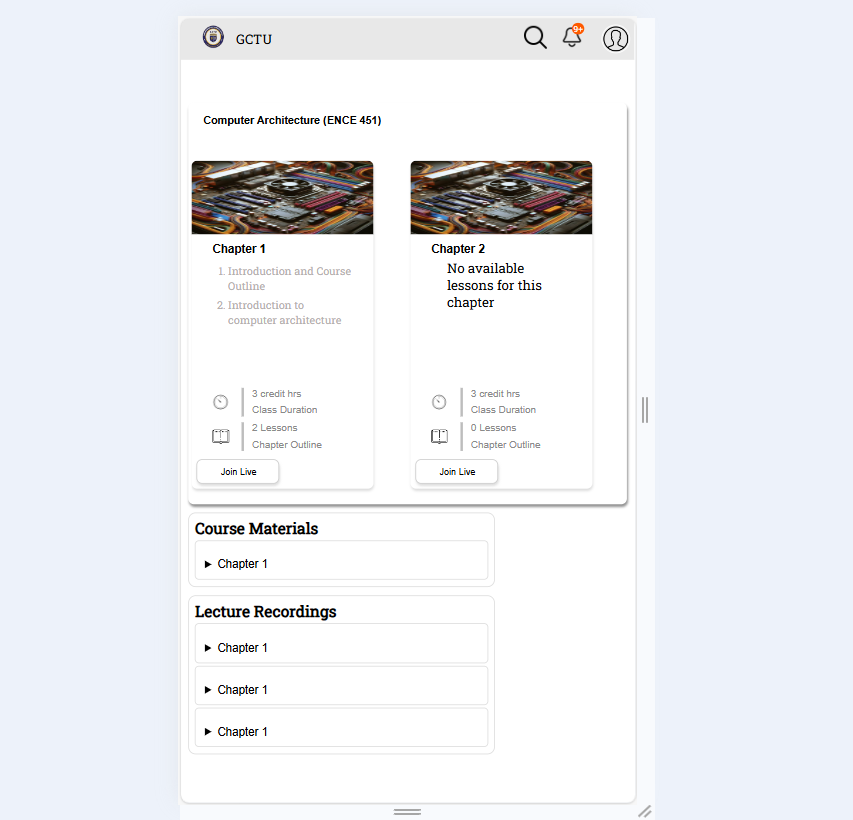
\includegraphics[width=1\textwidth]{figures/stud-c-deets.png}
      \caption{Students Course View Page UI (Solomon \& Avadzi, 2024)}
\end{figure}

\subsubsection{Waiting Room (for Both Students and Lecturers)}
The waiting room is a critical feature for managing the flow of live video conferencing sessions. Both students and lecturers enter the waiting room before the start of a meeting, where they can prepare for the session. The UI in the waiting room is designed to be minimalistic yet informative, displaying details about the upcoming session, including the start time, course name, and any relevant instructions. For students, the interface might include a notification that they are awaiting the lecturer’s arrival. For lecturers, it may offer options to review participant lists, adjust session settings, or send pre-session announcements. The waiting room helps ensure that all participants are ready and organized before the live session begins.\\

a.The waiting room for lecturer’s and meeting hosts.\\

\begin{figure}[H]
      \centering
      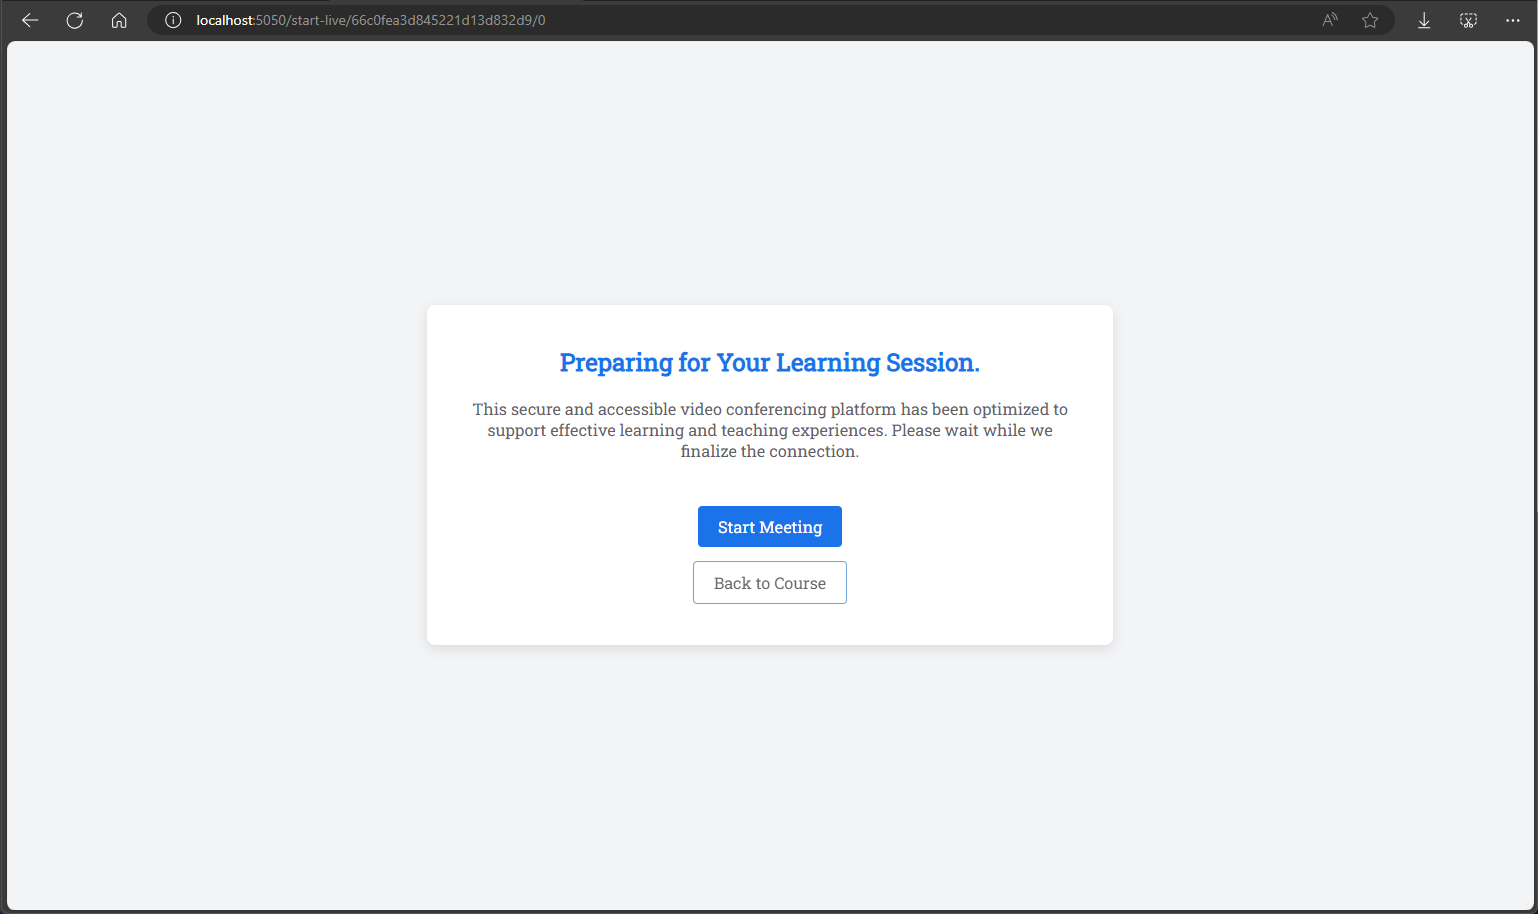
\includegraphics[width=1\textwidth]{figures/host-waiting-room.png}
      \caption{The Host's waiting room UI (Solomon \& Avadzi, 2024)}
\end{figure}

b.The waiting room for students.\\
\begin{figure}[H]
      \centering
      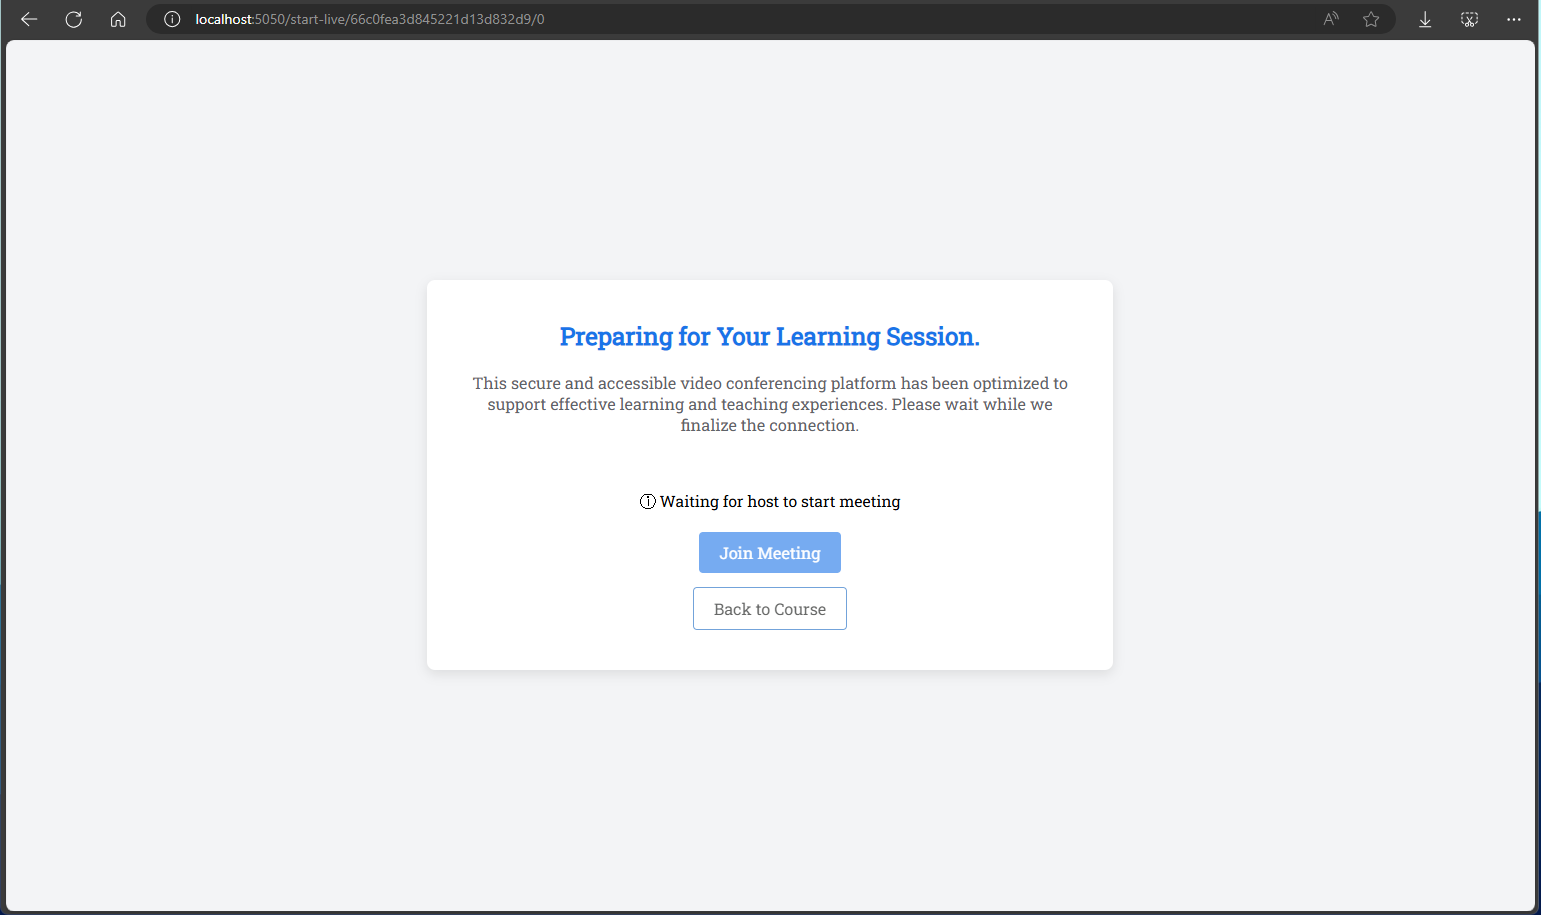
\includegraphics[width=1\textwidth]{figures/waiting-studs.png}
      \caption{Students waiting room UI (Solomon \& Avadzi, 2024)}
\end{figure}

\subsubsection{Meeting Room}
The meeting room is the core interface for live video conferencing sessions, where students and lecturers engage in real-time discussions and lectures. The UI here is designed to facilitate smooth communication, with video feeds displayed prominently for all participants. Essential controls for managing the meeting—such as muting/unmuting audio, turning the video on/off, screen sharing, and recording—are easily accessible. The meeting room also integrates features like a chat pane for text-based communication, a participants pane for managing attendee lists, and the ability to share educational materials during the session. The design ensures that both students and lecturers can focus on the content of the session without being distracted by the technical aspects of the platform.\\

a.Desktop view with the participants list open\\
\begin{figure}[H]
      \centering
      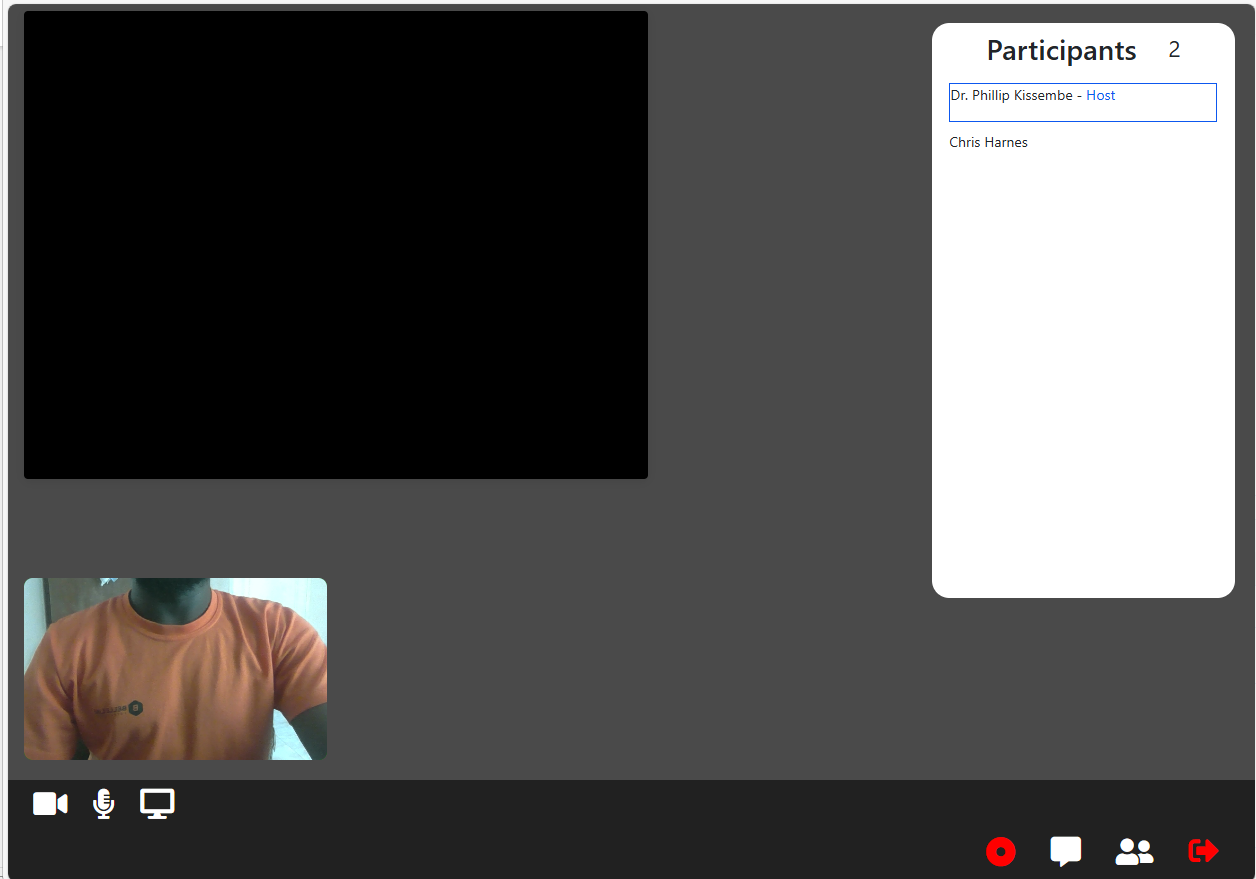
\includegraphics[width=1\textwidth]{figures/d-participants-open.png}
      \caption{Desktop view with the participants list (Solomon \& Avadzi, 2024)}
\end{figure}
b.Desktop view with chat pane open\\
\begin{figure}[H]
      \centering
      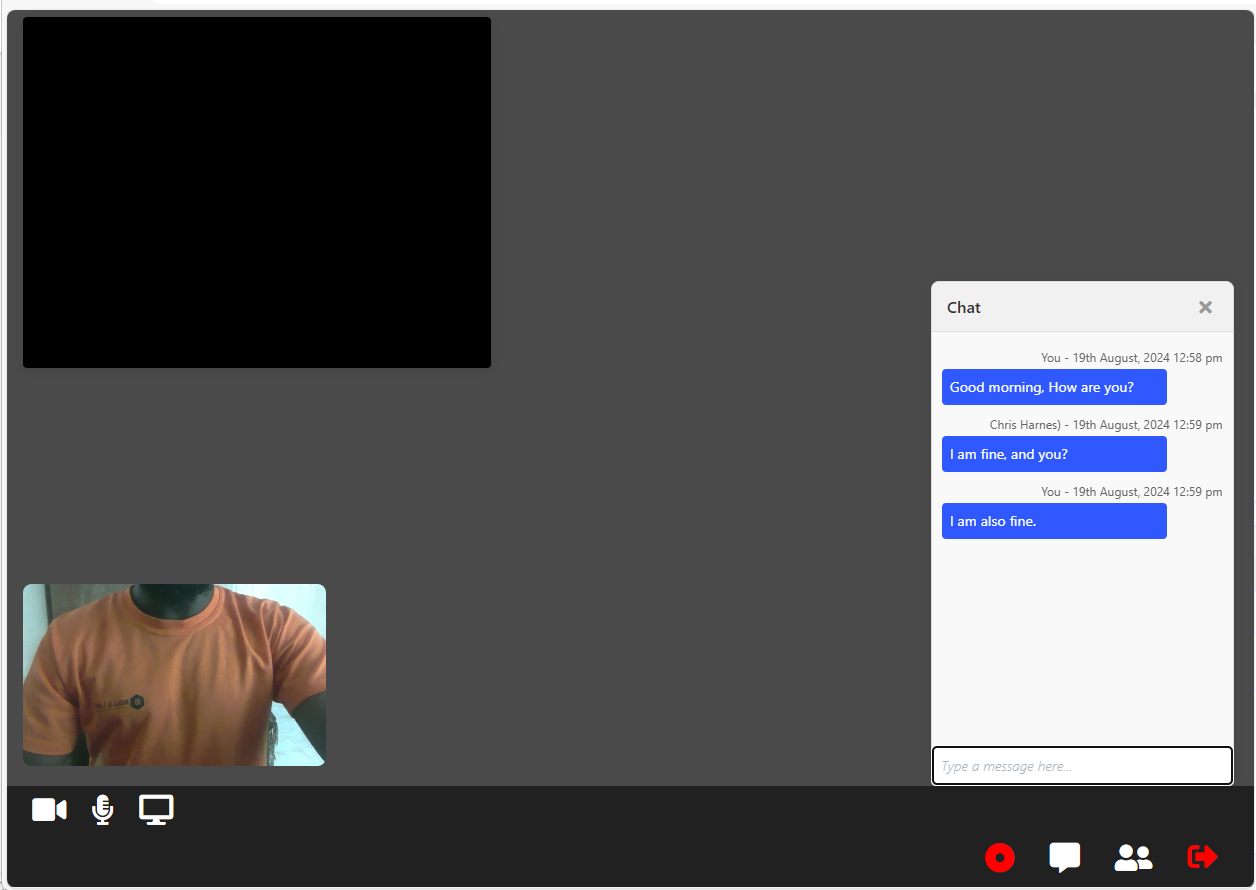
\includegraphics[width=1\textwidth]{figures/d-chats-open.png}
      \caption{Desktop view with chat pane  (Solomon \& Avadzi, 2024)}
\end{figure}
c.Desktop View with screen sharing active\\
\begin{figure}[H]
      \centering
      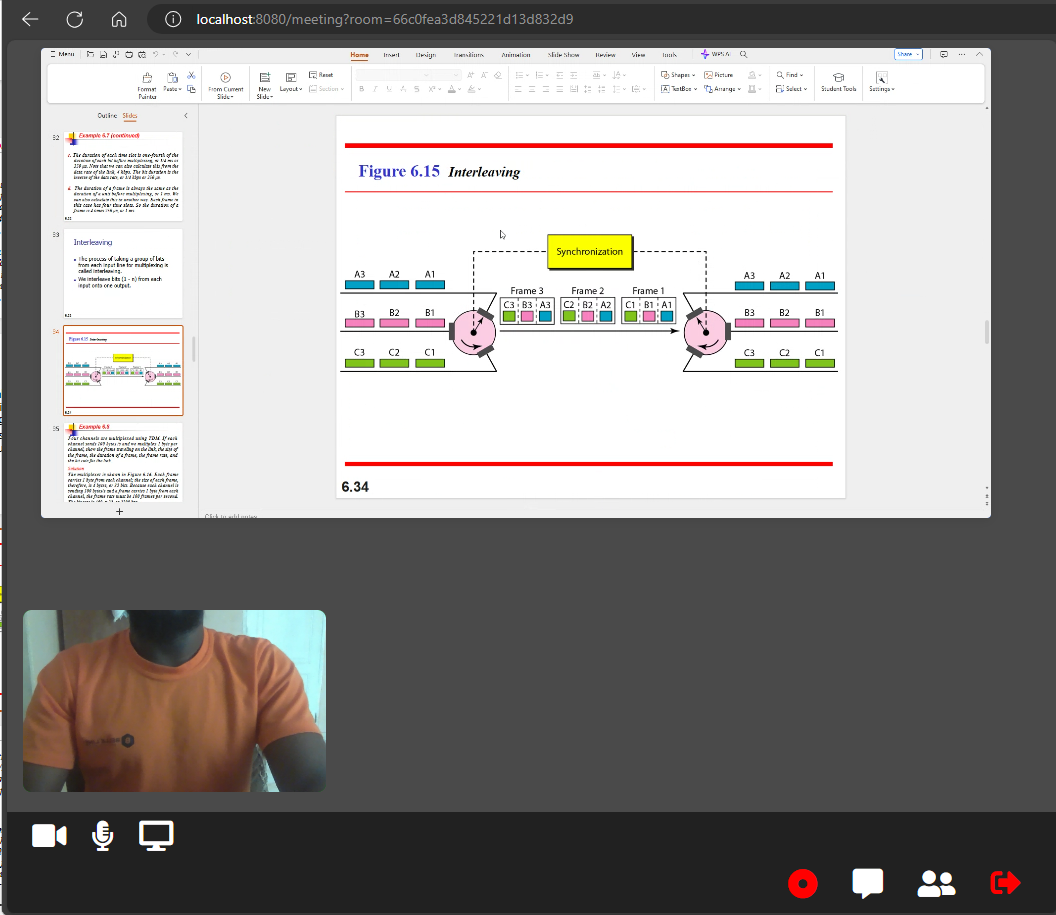
\includegraphics[width=1\textwidth]{figures/d-screenshare-open.png}
      \caption{Desktop View with screen sharing (Solomon \& Avadzi, 2024)}
\end{figure}
d.Mobile view with the chat pane open\\
\begin{figure}[H]
      \centering
      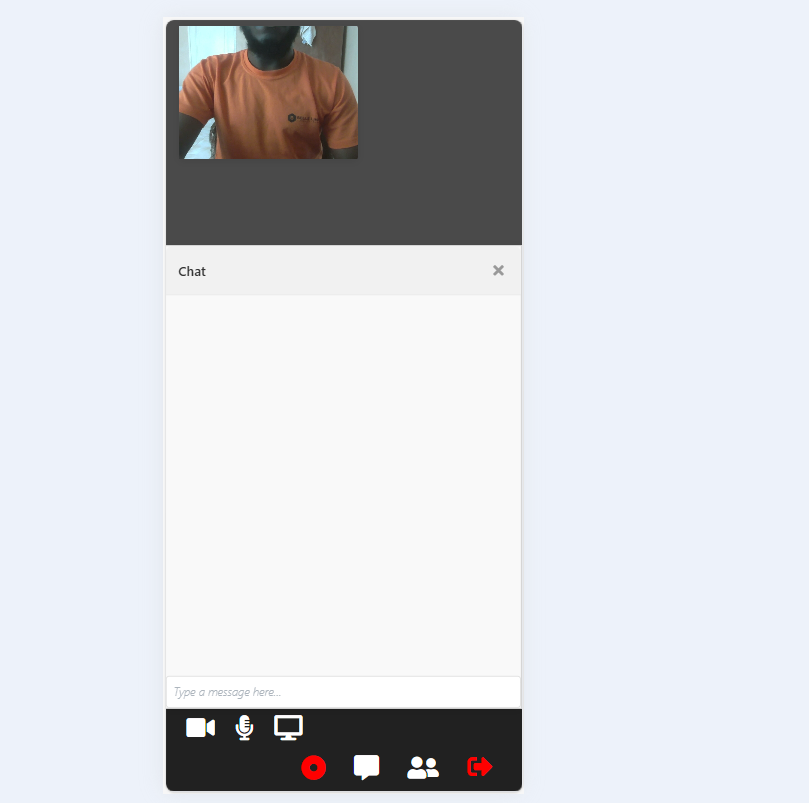
\includegraphics[width=1\textwidth]{figures/m-chats-open.png}
      \caption{Mobile view with the chat pane(Solomon \& Avadzi, 2024)}
\end{figure}
e.Mobile View with screen sharing active\\
\begin{figure}[H]
      \centering
      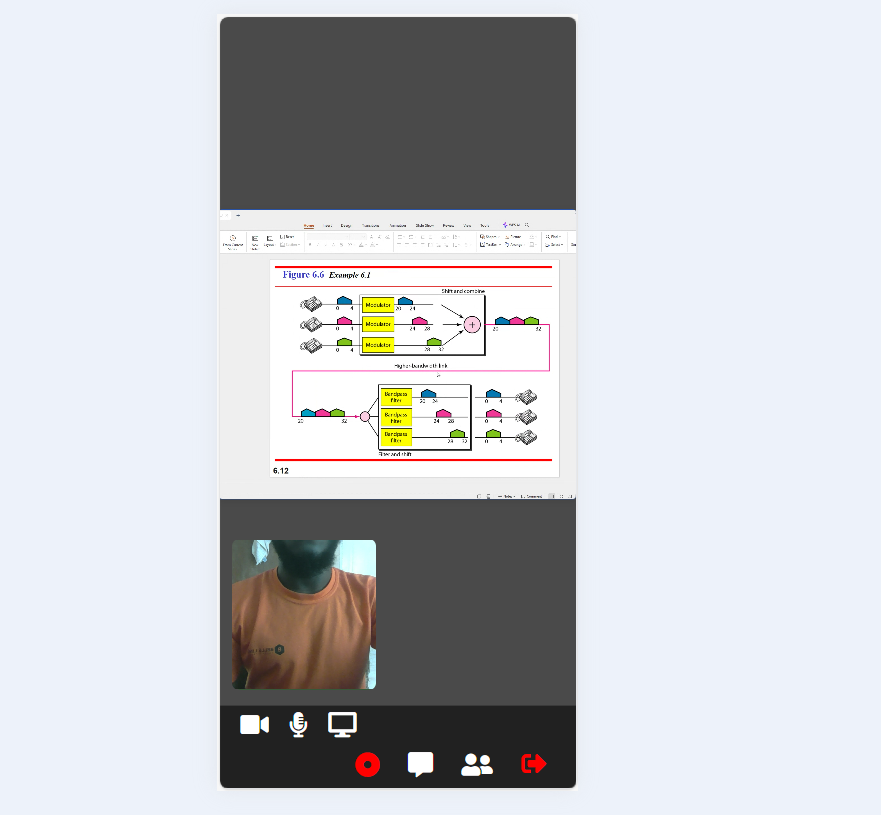
\includegraphics[width=1\textwidth]{figures/m-screenshare-open.png}
      \caption{Mobile View with screen sharing  (Solomon \& Avadzi, 2024)}
\end{figure}

\subsection{Evaluating and Testing}
The evaluation and testing phase of this project was grounded in a thorough analysis of existing works discussed in our literature review. By building on the insights and methodologies presented in these studies, we were able to systematically approach the evaluation process, ensuring that the system was tested against established benchmarks and best practices. This allowed us to identify key areas for enhancement, leading to significant modifications in the system's functionalities and performance. The application of these literature-based strategies not only improved the overall efficiency and user experience but also ensured that the system was aligned with current technological advancements and educational needs.\\

\subsection{Results}
The results of this project reflect a successful response to the challenges outlined in the problem statement. By leveraging the insights gained from our literature review and applying them strategically throughout the development process, we have created an integrated e-learning platform tailored specifically to the needs Ghana Communication Technology University (GCTU). The platform addresses key limitations in existing solutions, particularly the absence of built-in video conferencing capabilities in Moodle, and offers a more accessible and cost-effective solution for remote learning. The development and integration of a custom video conferencing feature have been particularly impactful. This feature not only bridges the gap left by Moodle but also enhances the overall functionality of the e-learning platform, making it more suited to the unique needs of GCTU. Through rigorous evaluation and testing, we have ensured that the platform is scalable, reliable, and capable of delivering high-quality education to students, regardless of their geographical location. Moreover, the platform effectively addresses the accommodation and accessibility challenges faced by GCTU, offering a viable alternative to physical classroom attendance. By reducing the need for on-campus presence, the platform alleviates the pressure on housing resources and allows students from remote areas to access quality education without the burden of long commutes. This contributes to creating a global learning community, enhancing the university's international recognition, and providing students with the opportunity to collaborate and learn in a more flexible and inclusive environment. The results demonstrate that the e-learning platform meets the objectives set out in the problem statement. It offers a comprehensive solution that not only meets the current needs of GCTU but also positions the university as a leader in leveraging technology to enhance educational accessibility and quality.\\

\subsubsection{The Benefits of the E-Learning Platform}
The implementation of this e-learning platform offers numerous benefits, both for Ghana Communication Technology University (GCTU) and its broader educational community. Firstly, the platform significantly enhances accessibility by enabling students in remote areas to participate in high-quality education without the need for physical attendance. This is particularly valuable in addressing the university's accommodation challenges, as it reduces the reliance on on-campus housing and alleviates the associated costs and logistical burdens on students. Additionally, the integration of a custom-built video conferencing feature directly addresses the limitations of Moodle and other existing Learning Management Systems. This capability facilitates real-time interaction between instructors and students, enriching the learning experience through immediate feedback, collaborative learning, and a more engaging educational environment. Unlike costly third-party solutions, this integrated feature is designed to be cost-effective, aligning with GCTU's financial constraints while providing a sustainable long-term solution. The system also enhances the university’s global reach by enabling it to offer courses and programs to students worldwide. This not only increases the university's international recognition but also fosters a global learning community where students from diverse backgrounds can collaborate, share knowledge, and learn together. Furthermore, the platform supports the university’s mission of innovation by providing a customizable and scalable solution that can evolve with the institution's needs. This flexibility ensures that GCTU can continue to adapt to new educational trends and technologies, maintaining its competitive edge in the higher education landscape. Overall, the system empowers GCTU to provide a more inclusive, flexible, and sustainable educational experience, benefiting both students and faculty by overcoming the limitations of traditional learning models and enhancing the university's capacity to deliver quality education on a global scale.\\

\subsection{Chapter Summary}
This chapter provides a comprehensive examination of the e-learning platform's development, focusing on the user interface, evaluation, testing, and results of the implemented video conferencing feature. The design of the project has been successfully completed, emphasizing its video conferencing and communication capabilities. The platform’s video and audio sharing features were rigorously tested across various devices, including laptops and mobile phones, with satisfactory results. Additionally, the text messaging functionality was tested and met performance expectations. Participants in the testing phase highlighted the simplicity and user-friendliness of the interface, which contributes to a seamless and engaging educational experience. The chapter also details how insights from the literature review informed system refinements, leading to improvements in functionality and performance. By effectively addressing the limitations of existing solutions, the platform enhances accessibility, reduces costs, and supports GCTU’s mission of global engagement. Overall, this chapter demonstrates that the platform meets technical requirements while providing an intuitive and effective user experience, aligning with the project's goals and objectives.\\ \newpage

\begin{center}
      \section*{CHAPTER FIVE}
      \section{CONCLUSION, LIMITATION AND RECOMMENDATION}
\end{center}

\subsection{Overview}
This is the final chapter in this project work. In this chapter, we conclude and finalize the purpose and workings of this project. We also make recommendations for researchers who are interested in making this project better in the future.\\

\subsection{Conclusion}
In this project, we developed and implemented an Enhanced E-Learning Platform designed to significantly improve the interactive educational experience. The platform includes advanced features such as video conferencing, a centralized repository for accessing learning materials, assessment tools, and an embedded chat system to facilitate real-time communication and engagement among students and instructors. The primary objective is to create a robust and interactive learning environment that enhances the educational experience beyond traditional methods. The project has been successfully implemented, providing a comprehensive solution for virtual classrooms and interactive learning sessions all on one platform.\\

\subsection{Limitations}
\begin{enumerate}
      \item Challenges in Recording Video Sessions:\\
      We faced significant difficulties in effectively recording video sessions on our servers. The technical issues encountered will prevent particpants  to download the class meetings right after it ends.\\

      \item Live Stream Limitations:\\
      The current system is unable to support multiple users having their video and audio enabled simultaneously during a live stream. This restriction affects the overall quality and usability of the live streaming experience for participants.\\
\end{enumerate}

\subsection*{Recommendations}
\begin{enumerate}
      \item  Recording Video Sessions:\\
      To address the challenges with server-side recording, it is recommended that each participant record the video sessions on their individual computers. This approach will help ensure that recordings are available and can be easily managed without relying on server capabilities.\\
      \item Managing Live Streams:\\
      To improve the efficiency and quality of live streaming, it is recommended that only the host (lecturer) should only have their audio and video enabled during the entirety of the session, while other participants enable theirs as needed. This adjustment will help the system handle multiple participants more effectively, reducing the risk of technical issues and ensuring a smoother experience for everyone involved.\\
\end{enumerate}

\newpage
\bibliographystyle{IEEEtran}
\bibliography{references.bib}
\addcontentsline{toc}{section}{References}
\end{document}